\documentclass[../main.tex]{subfiles}
	% THE RASPBERRY PI AND THE TEST BED
\begin{document}

Talk about the RPi and test bed.

%%%%%%%%%%%%%%%%%%%%%%%%%%%%%%%%%%%%%%%%%%%%%%%%%%%%%%%%%%%%%%%%%%%%%%%%%%%%%%%%%%%%%%%%%%%%%%%%%%%%%%%%%%%%%%%%%%%%%%%%%%%%%%%%%%

\section{Fundamentals}

The Raspberry Pi is a simple, affordable ARM-based computing module. It has General Purpose Input/Output (GPIO) pins which it can use to interface with stuff.\\

It is run using a Linux-based operating system called Raspbian which is available for download from the Raspberry Pi official website \cite{lib_Raspbian}.\\

The main chip on the board is the Broadcom BCM2835.
The Pi's pins can either be numbered as pin 1-40 going through them sequentially in layout, this is the BOARD numbering scheme, or they can be referred to by their Broadcom pin numbers with the BCM numbering scheme.
The second scheme numbers the available GPIO pins in the range 2-27 (Pins 0 and 1 are reserved for system use).

\todo[inline,color=blue!20]{Write Raspberry Pi Fundamentals -- and take a better picture}

\begin{figure}[ht]
	\centering
	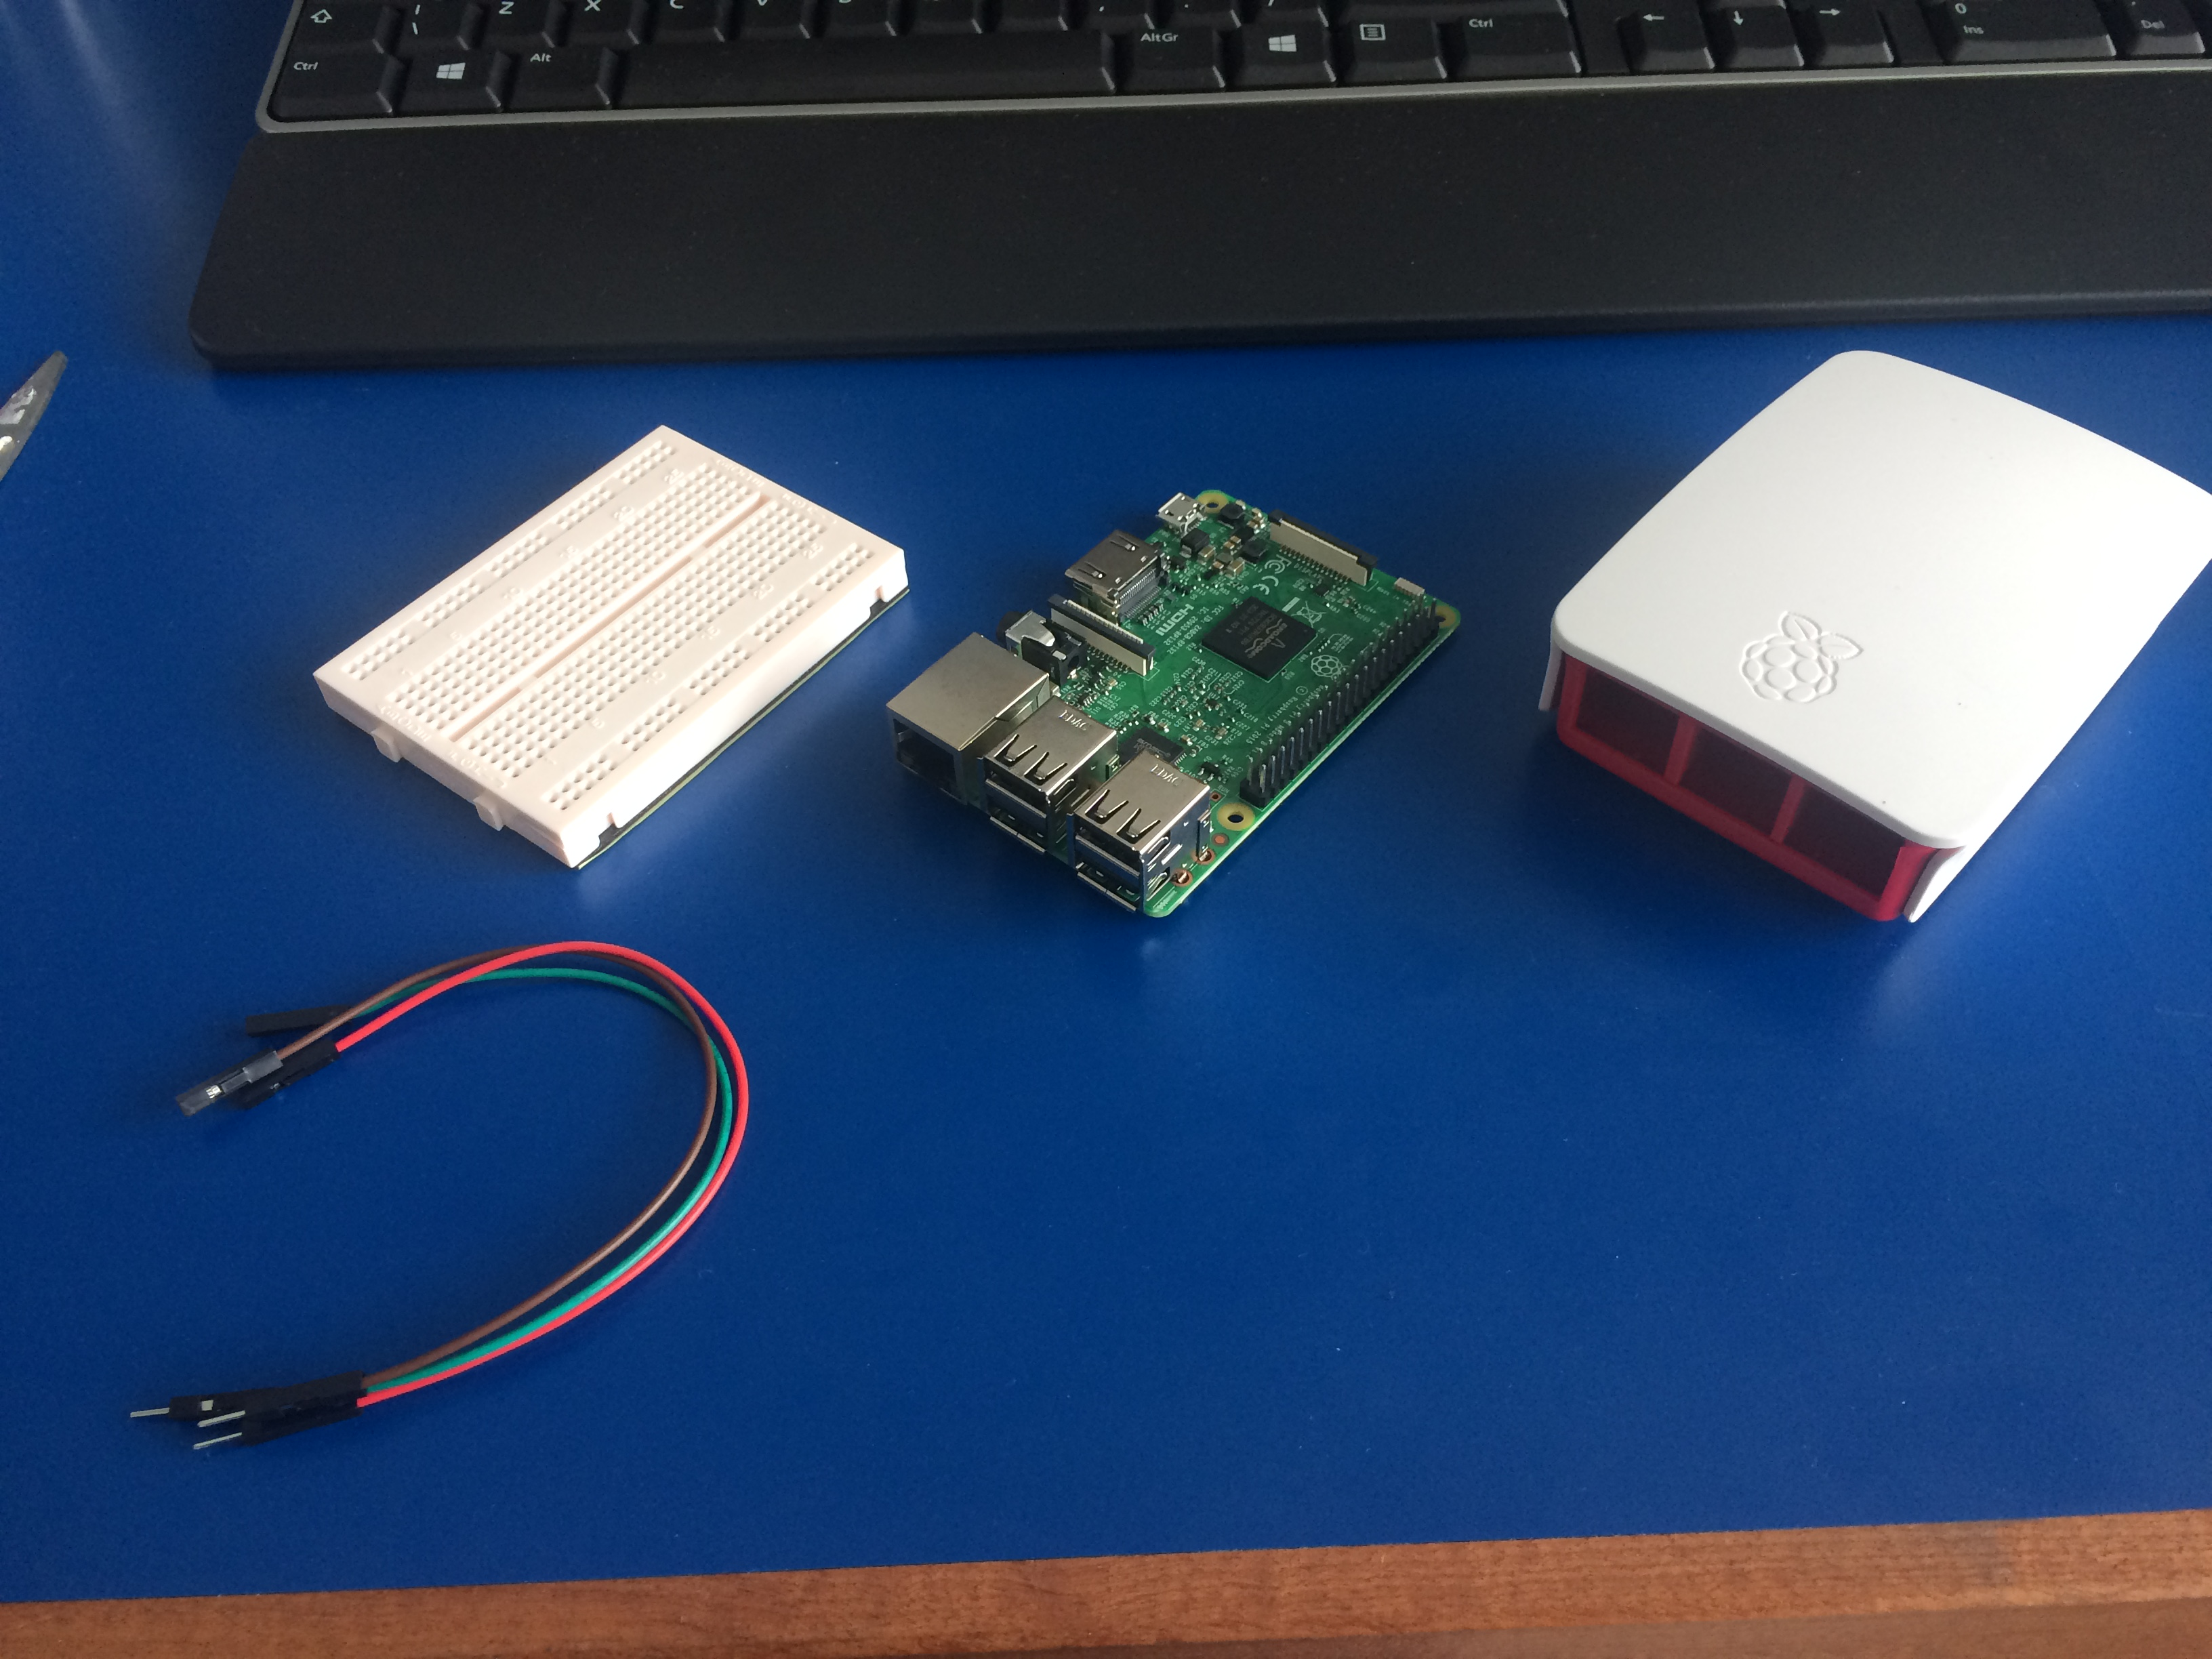
\includegraphics[width=0.6\textwidth]{Raspberry_Pi.jpg}
	\caption{The Raspberry Pi}
	%\label{fig_}
\end{figure}

\subsection{Setting up the Raspberry Pi}

The Raspberry Pi can be interfaced with in a number of ways, but first it needs to be set up with its operating system on the SD card \cite{web_SetupRaspbian}.
Raspbian can be accessed via the command line - typing in commands - or through an X Window similar to Windows OS.
Either of these options can be used by connecting a screen, keyboard and mouse to the Pi, but this is not always available, so it is useful to have Secure Shell (SSH) set up for the command line, and Virtual Network Computing (VNC) for the X Window.
Secure Shell is necessary regardless as it is used in the test bed execution.
When actually using both Raspberry Pis in the test bed, both of them will be running in command line mode as this saves resources, although during development, VNC or a screen using the X Window makes it much easier to test and edit code.
In the test bed, the Transmitter Pi will be connected to a screen and peripherals in command line mode, and then it will start the Receiver via SSH, which will run headless (without a screen or control peripherals) and receive the data, process and output it, and store information about the run in a log file which can be accessed later or again through SSH.\\

\missingfigure{A flowchart that describes the set-up procedure could be useful.}

Once the operating system is written to the SD card, SSH can be enabled by creating an empty file \textit{ssh} in the main portion of the card before putting it in the Raspberry Pi (for setup using a screen and peripherals, this can be turned on in the configuration settings).
Now an Ethernet cable can be connected from a computer to the Pi and it can be logged into.
A program such as PuTTY \cite{lib_PuTTY} for Windows can be used, with \textit{pi@raspberrypi.local} as the host name so the IP address is not needed.
The standard login is \textit{username: pi} and \textit{password: raspberry}.
The command \textit{sudo raspi-config} accesses the configuration settings where the file system can be expanded to the whole SD card, and other utilities such as Wi-Fi and VNC can be turned on.
Again, all utilities except for SSH should be turned off when using the final test bed to improve performance of the devices.
Once the Pi is connected to Wi-Fi and the IP address is known, it can be accessed remotely via the free RealVNC VNC Viewer \cite{lib_RealVNCViewer} and the X Window can be started with the command \textit{startx} if it is not already set to open the X Window on startup in the configuration settings.
This access can be made permanent by setting the Pi to have a static IP address or with a free RealVNC account which lets it be accessed independent of the IP address.\\
\todo[inline,color=green!40]{Inline code reference should look like inline code not just italics ideally}

With full control of the Pi, all that is needed is to download all of the libraries and software used by the test bed and clone the GitHub repository with its code.
The Python version used is 3.6.4.
\todo[inline]{Double check Python version of Pis is correct}
and as the Raspberry Pi has Python 2 and 3, pip - the Python package manager - is called as pip3 for python3.
Any dependencies not in this list give clear instructions as to how they are downloaded when this list is run line by line.\\

\todo[inline,color=green!40]{Create new format (and inline for above) called "shell"} IF I NEED TO AND HAVE TIME
\lstset{style=python}
\begin{lstlisting}[caption=Libraries and Packages Required for the Test Bed]
	sudo apt-get update
	
	sudo apt-get install vpnc
	sudo apt-get install libffi6 libffi-dev python-dev
	sudo pip3 install cryptography paramiko
	
	sudo apt-get install libatlas-base-dev
	sudo pip3 install numpy imageio
	sudo apt-get install pigpio
	
	sudo apt-get install git
	cd "<Path for the code e.g. /pi/home/Documents/>"
	git clone https://github.com/CamEadie/4YP_PiCom

	sudo apt-get update && sudo apt-get upgrade && sudo apt-get dist-upgrade

	# Used in Transmit_Binary_Data(): import RPi.GPIO as GPIO
	# ... This library is already included in the Raspberry Pi
	# ... Only for OOK transmission which uses Python not C
	# Used in Check_Input_Masks(): from RPiSim.GPIO import GPIO
	# ... pip GPIOSimulator (or pip3 if necessary)
	# ... Only works in Windows, simulates Raspberry Pi pins (use like RPi.GPIO commands)
\end{lstlisting}

Included are the following, as well as their dependencies:

\begin{itemize}
	\item VPNC - VPN software used to access Oxford VPN in order to use the OWL Wi-Fi network \cite{lib_VPNC}
	\item Paramiko - Python library used for SSH to start the receiver \cite{lib_Paramiko}
	\item NumPy - Python library used for easier array manipulation as well as interface with images \cite{lib_NumPy}
	\item imageio - Python library used to read and save image files as NumPy arrays \cite{lib_imageio}
	\item pigpio - C library used to interface with the GPIO pins \cite{lib_pigpio}
	\item Git - Version control software which also allows for the cloning of the project code to any device \cite{lib_Git}
\end{itemize}

\clearpage

%%%%%%%%%%%%%%%%%%%%%%%%%%%%%%%%%%%%%%%%%%%%%%%%%%%%%%%%%%%%%%%%%%%%%%%%%%%%%%%%%%%%%%%%%%%%%%%%%%%%%%%%%%%%%%%%%%%%%%%%%%%%%%%%%%
	
\section{Test Bed Architecture}

The test bed comprises the two Raspberry Pis and a number of chips to provide the functions required for more advanced modulation schemes.
This is built up as three arrangements with increasing complexity.
The first is the Pis connected together by two wires, a serial data line and a clock line (Figure \ref{fig_OOK Architecture}).
This arrangement is similar to that used for an $I^2C$ bus, however the code written for this form of communication does not rely on any available modes of serial interfacing because it needs to be extensible to the parallel communication in the next arrangements.
The second arrangement is used for Pulse Amplitude Modulation schemes.
It uses a single parallel Digital Analogue Converter (DAC) connected to the transmitter which transmits to a parallel Analogue Digital Converter connected to the receiver, allowing for multi-level signals to be transmitted between the two devices.
The final arrangement extends the set-up to two DACs and two ADCs.
These signals are then multiplied by a sine wave and a cosine wave respectively, and can be separated due to the orthogonality of the two signals at the receiver.
This arrangement is used for Quadrature Amplitude Modulation as well as Orthogonal Frequency Division Multiplexing.\\

\begin{figure}[ht]
	\centering
	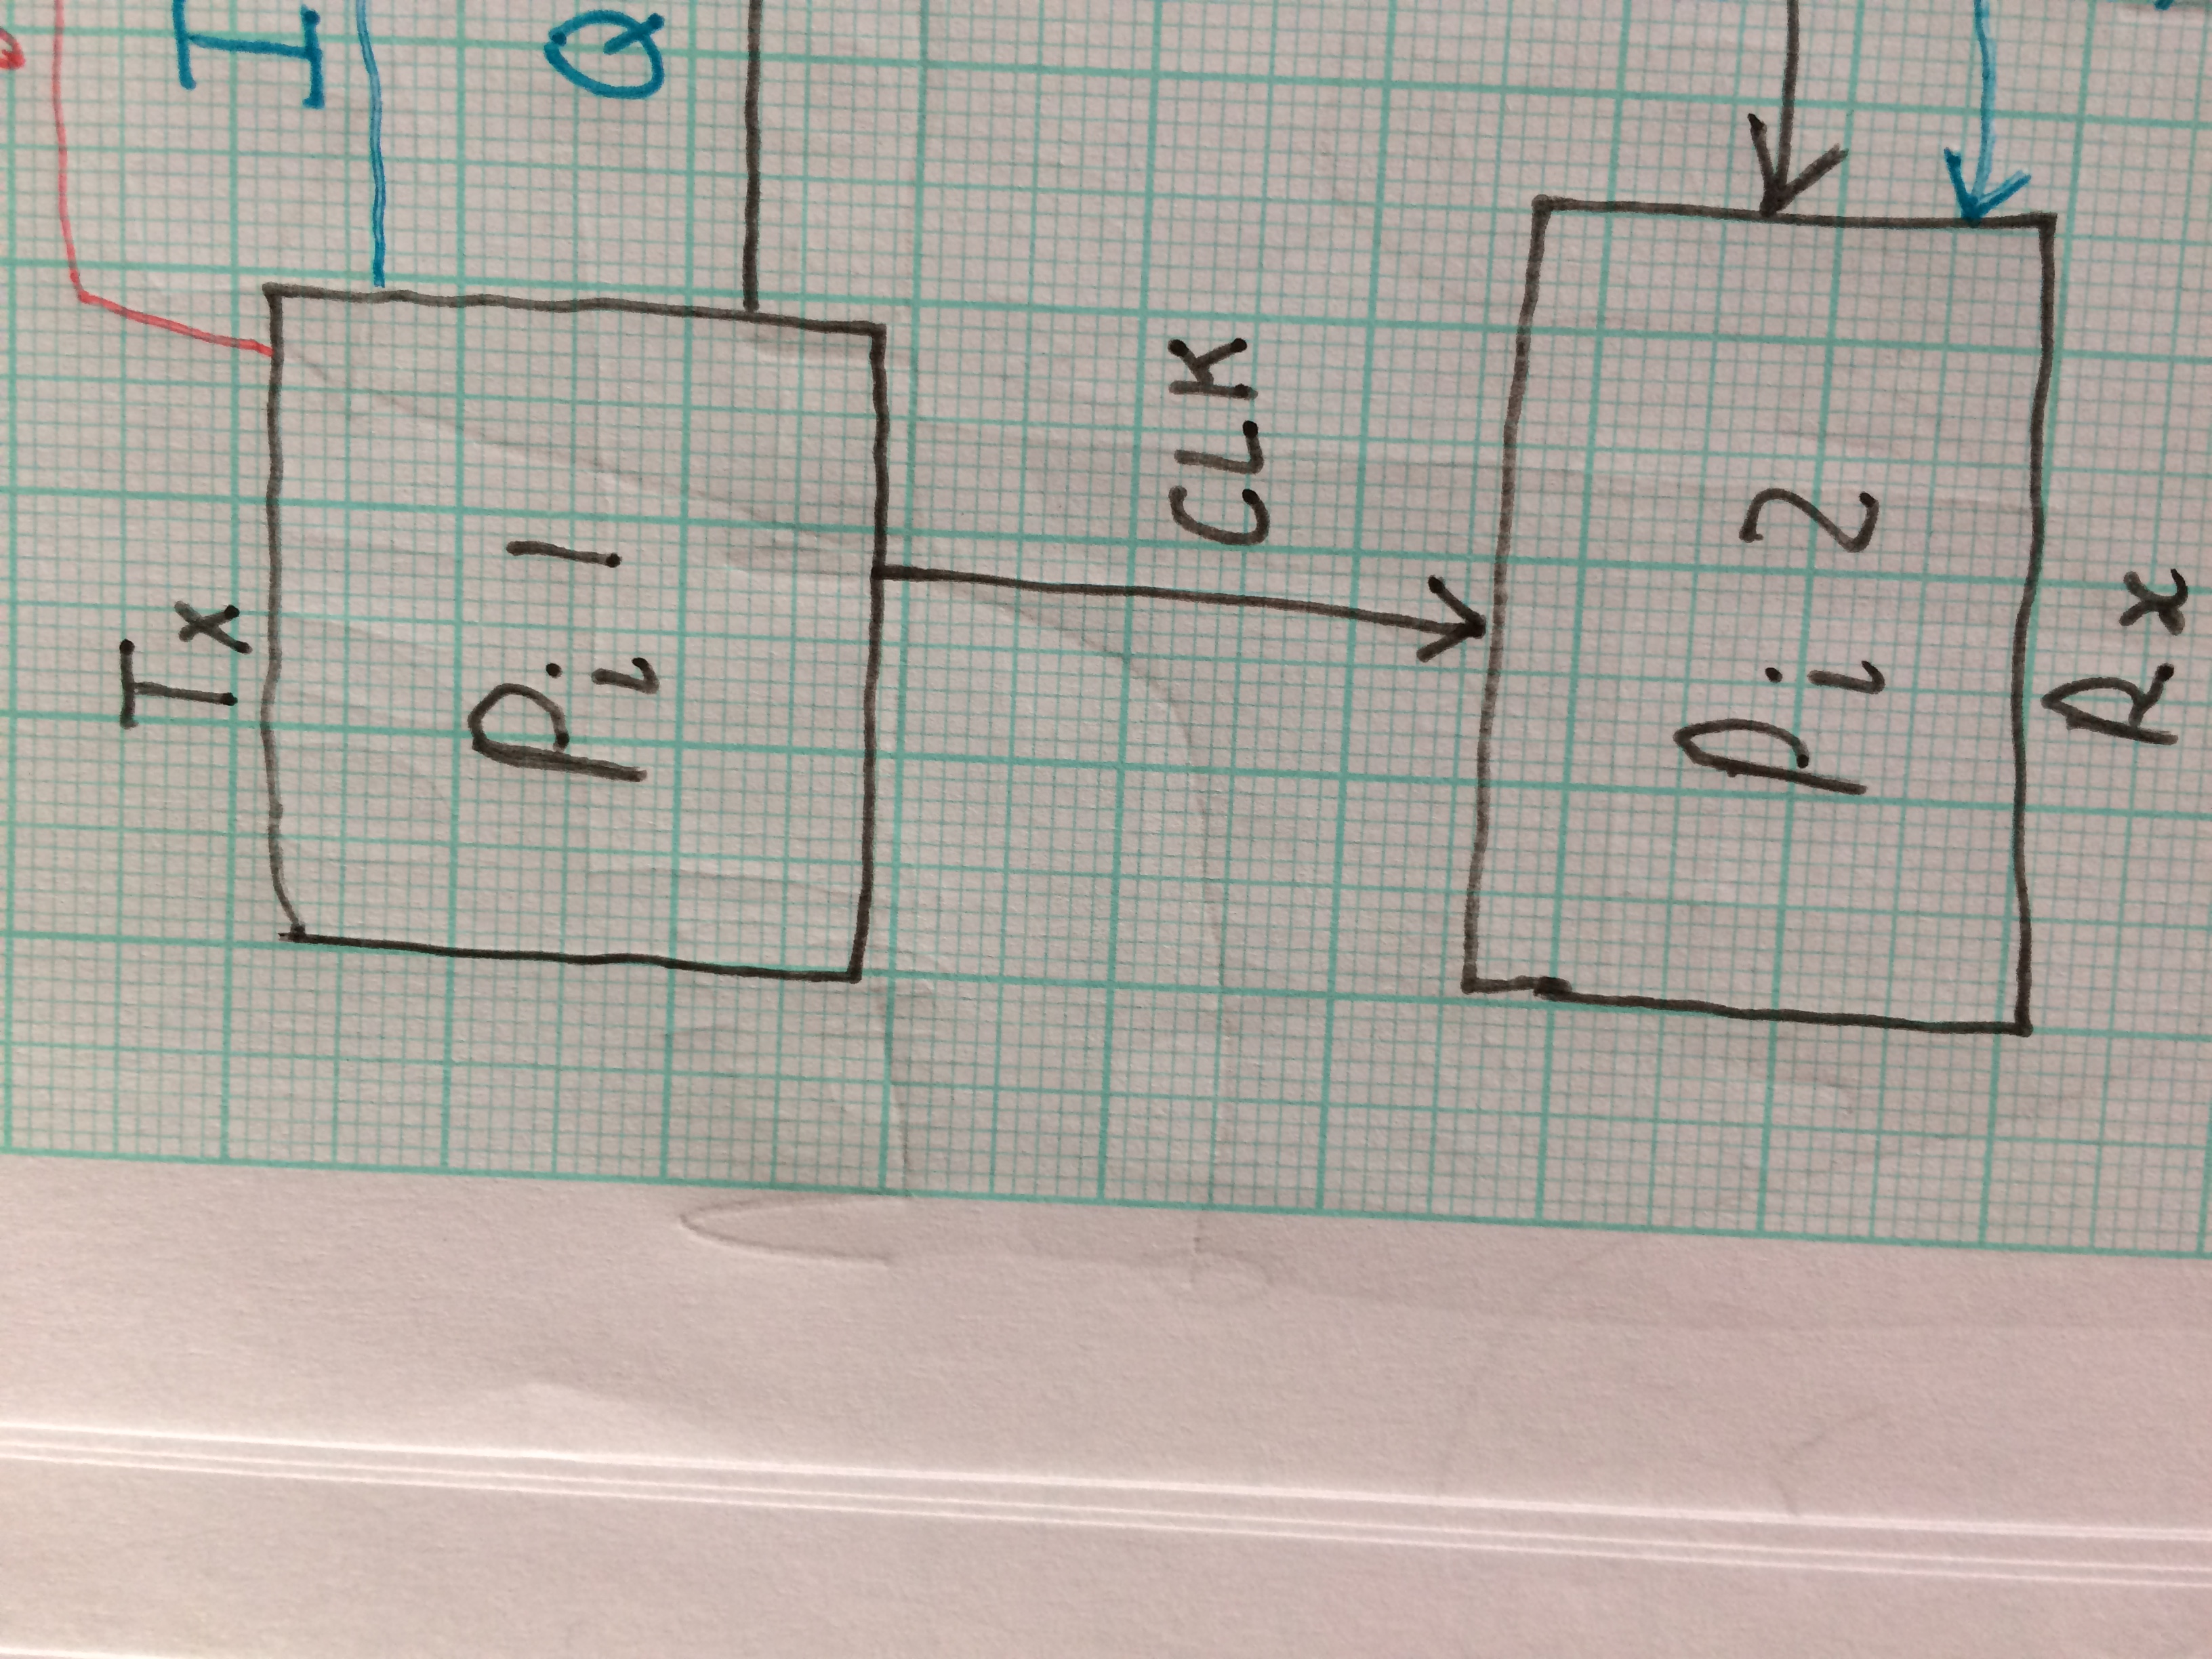
\includegraphics[width=0.5\textwidth]{OOK_Architecture.jpg}
	\caption{Test Bed Set-up For On-Off Keying}
	\label{fig_OOK Architecture}
\end{figure}

\subsection{Digital Analogue Converter}

The Digital Analogue Converter used is the AD5424, an 8-bit CMOS current output DAC with an easy interface to microcontrollers.
It has a \SI{17}{\nano\second} write cycle and a maximum update rate of \SI{20.4}{MSPS}. % Mega Samples Per Second
There are possible configurations in the data sheet using an inverting operational amplifier to produce the output, however due to the single supply and difficulties finding low-power operational amplifiers which provide rail-to-rail output for a 5V single supply, this was avoided where possible.
The Read/Write ($R/\overline{W}$) pin is pulled low permanently so the chip is in write mode; read back of the parallel digital outputs is not required.
The Chip Select pin ($\overline{CS}$) needs a falling edge and a rising edge to complete a write cycle, where the rising edge loads new parallel data, so this is connected to the clock pin of the Raspberry Pi.
Layout of the connections to the Pi are in the Figure \ref{fig_DAC Layout}.\\

\begin{figure}[ht]
	\centering
	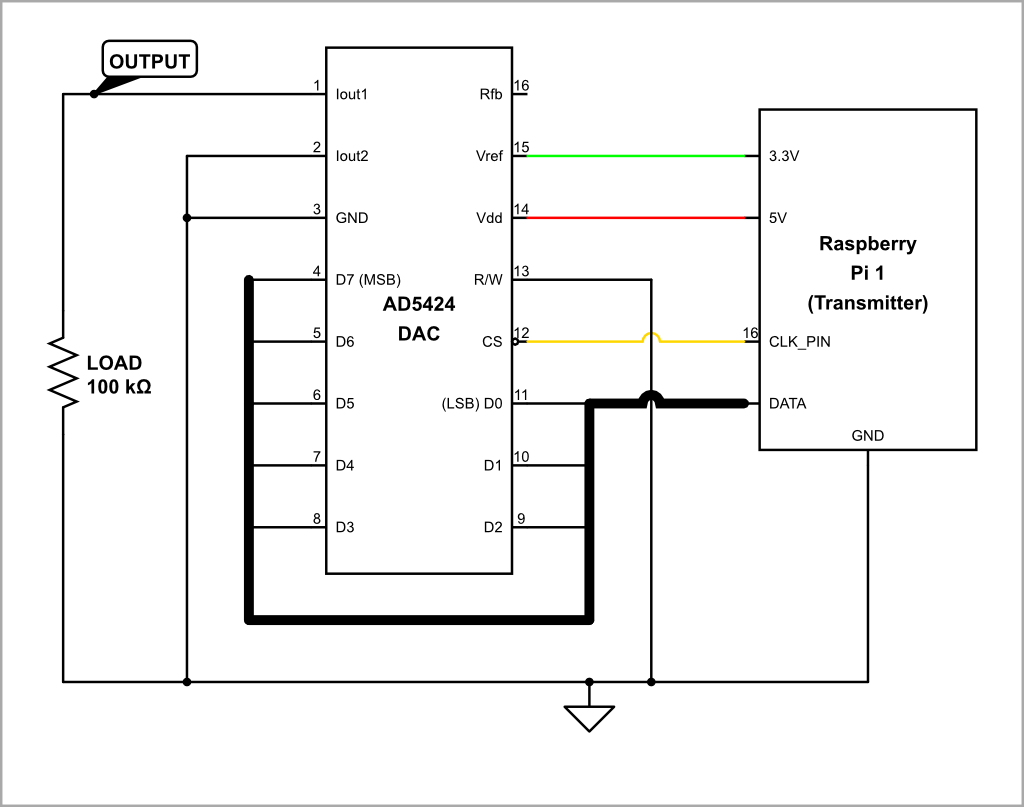
\includegraphics[width=0.8\textwidth]{ad5424.png}
	\caption{Layout of the Digital Analogue Converter}
	\label{fig_DAC Layout}
\end{figure}

\subsection{Analogue Digital Converter}

The Analogue Digital Converter used is the ZN448, 
\todo[inline,color=blue!20]{Write up layout of the ADC and more on Multiplier and other parts}

\begin{figure}[ht]
	\centering
	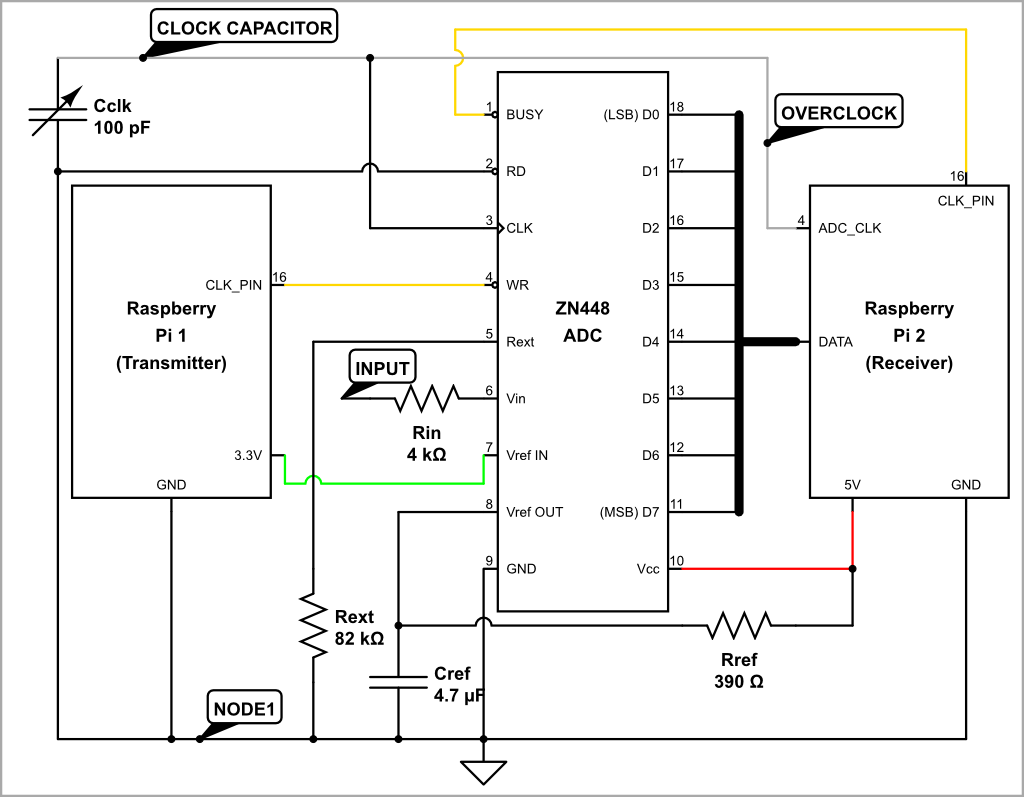
\includegraphics[width=0.8\textwidth]{zn448.png}
	\caption{Layout of the Analogue Digital Converter}
	\label{fig_ADC Layout}
\end{figure}

\begin{figure}[ht]
	\centering
	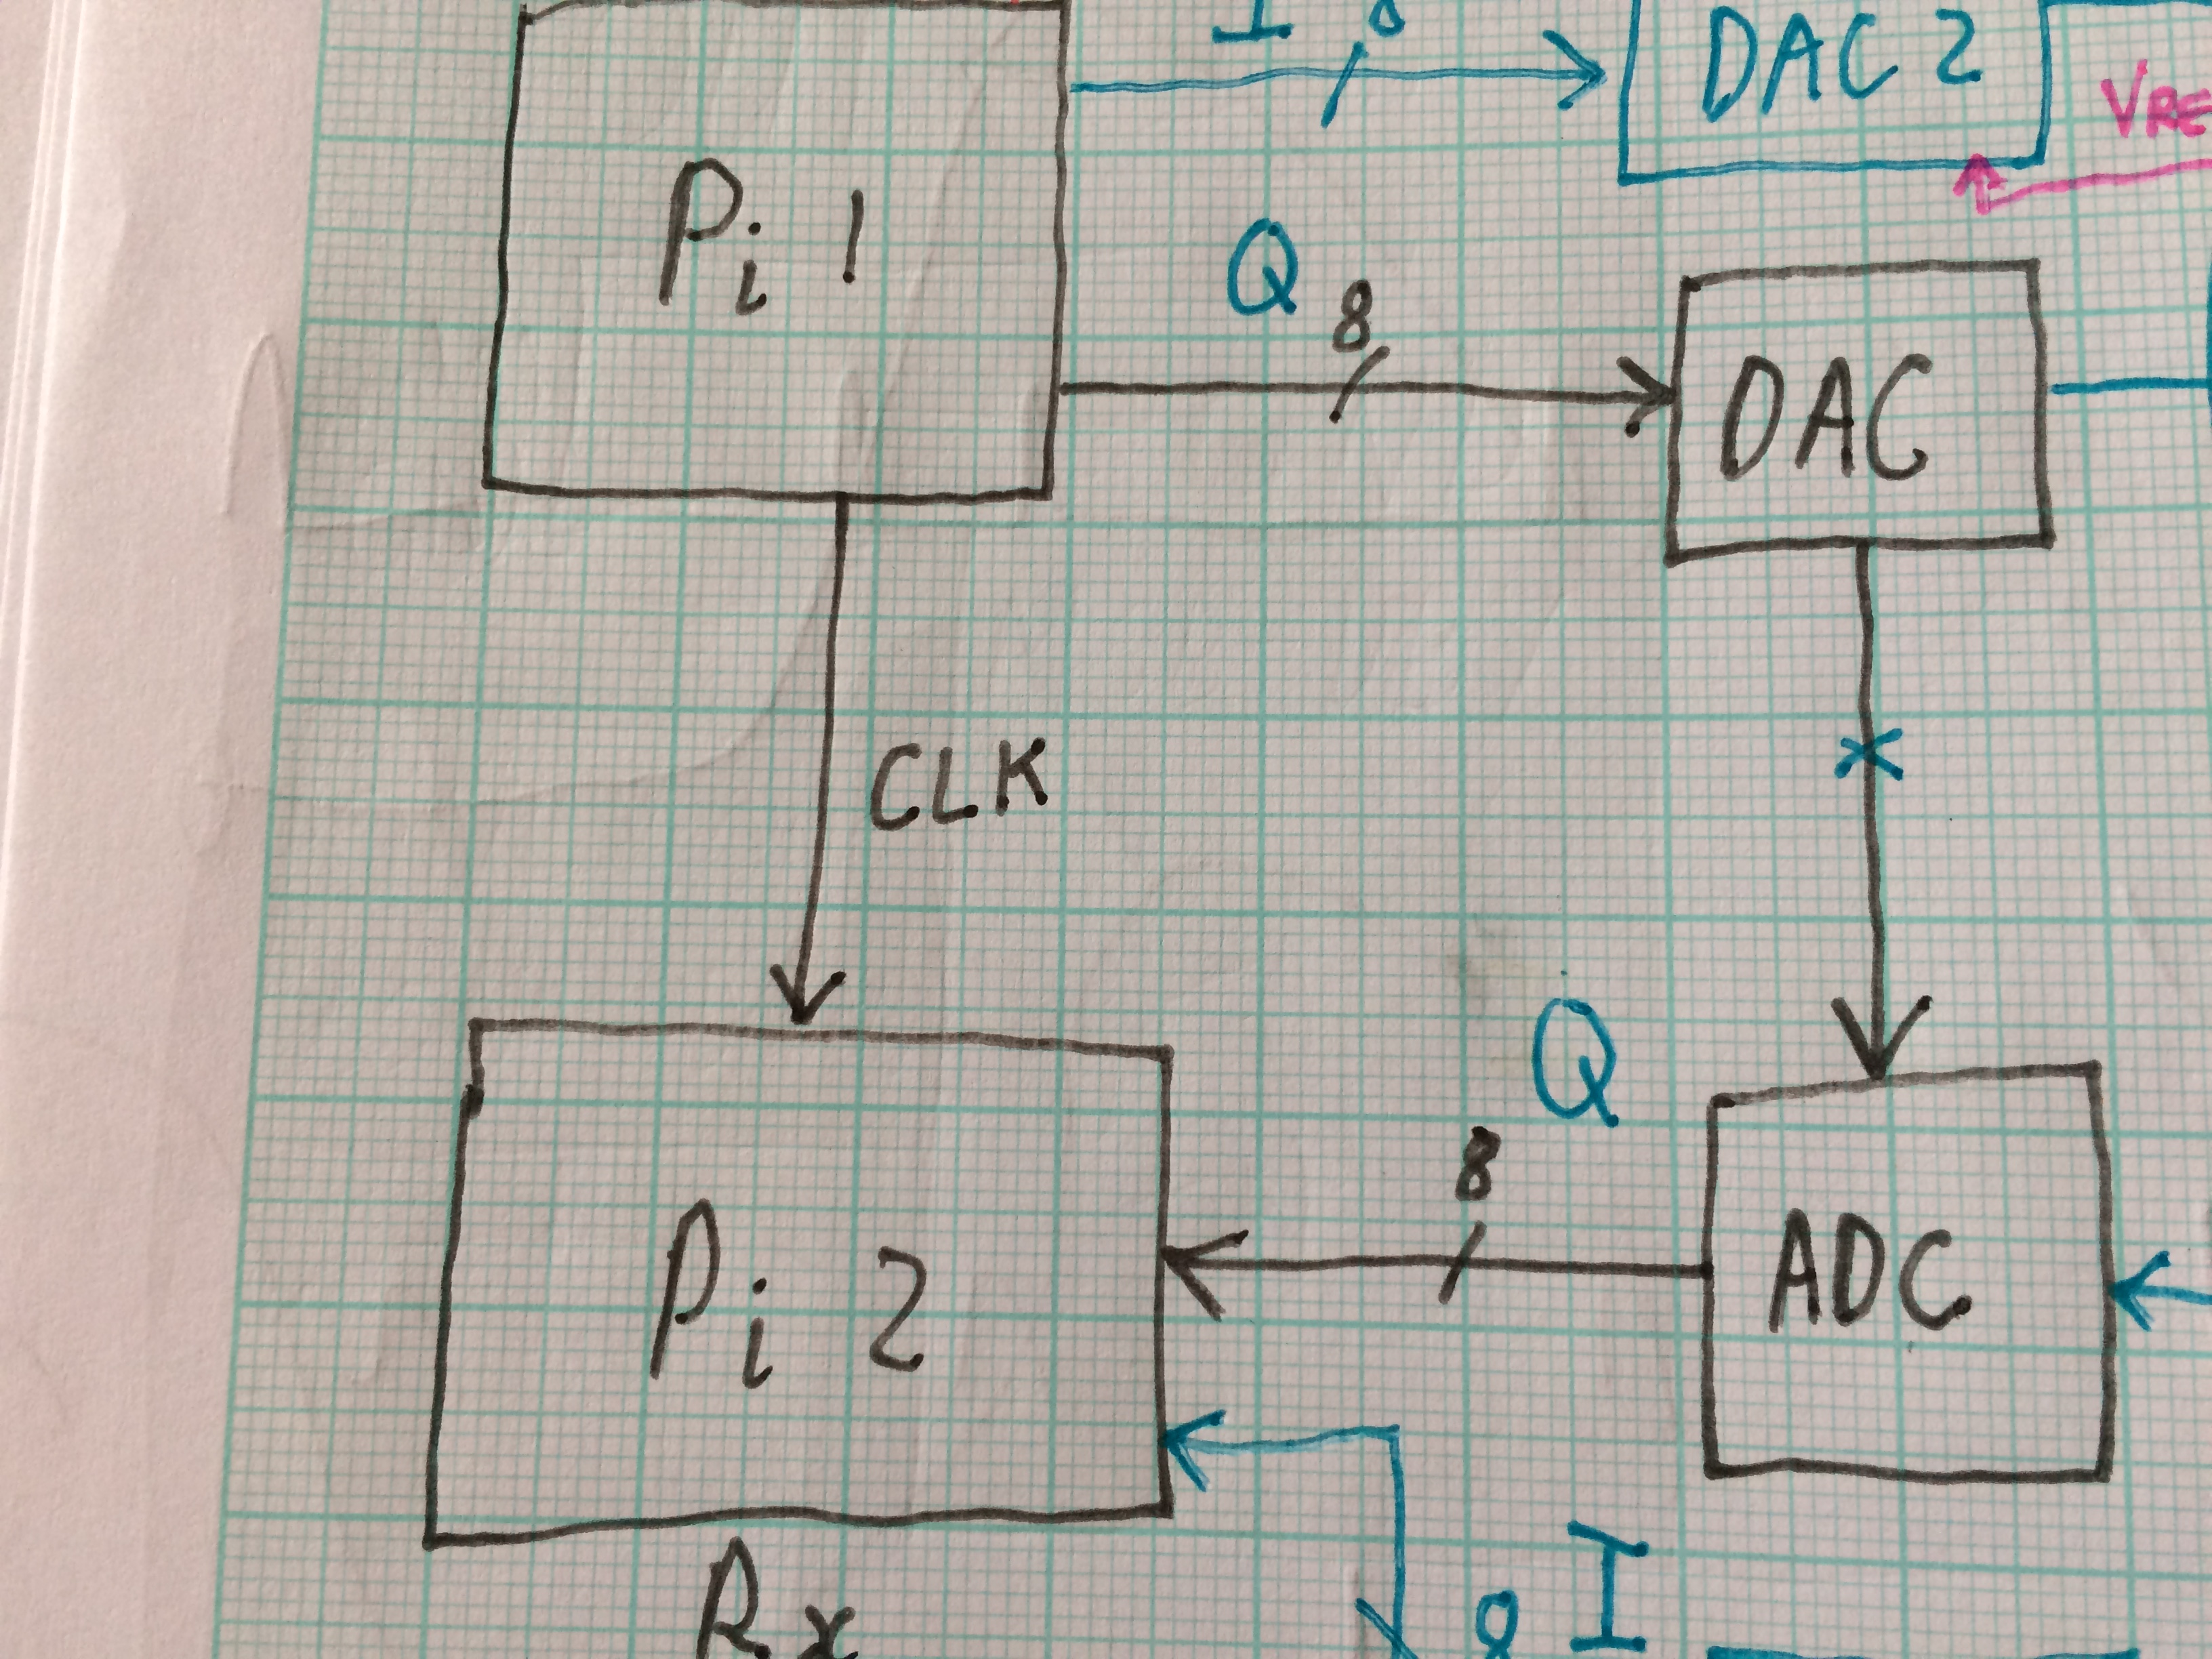
\includegraphics[width=0.4\textwidth]{PAM_Architecture.jpg}
	\caption{Layout of Test Bed for Pulse Amplitude Modulation}
	%\label{fig_}
\end{figure}

\subsection{Multiplier} \label{sec_Multiplier}

This section still needs the technical specifications and layout in the test bed of the multiplier.

\todo[inline]{Depending whether it's doable, include  this section without multipliers on transmitter, pseudo ground on output}

\begin{figure}[ht]
	\centering
	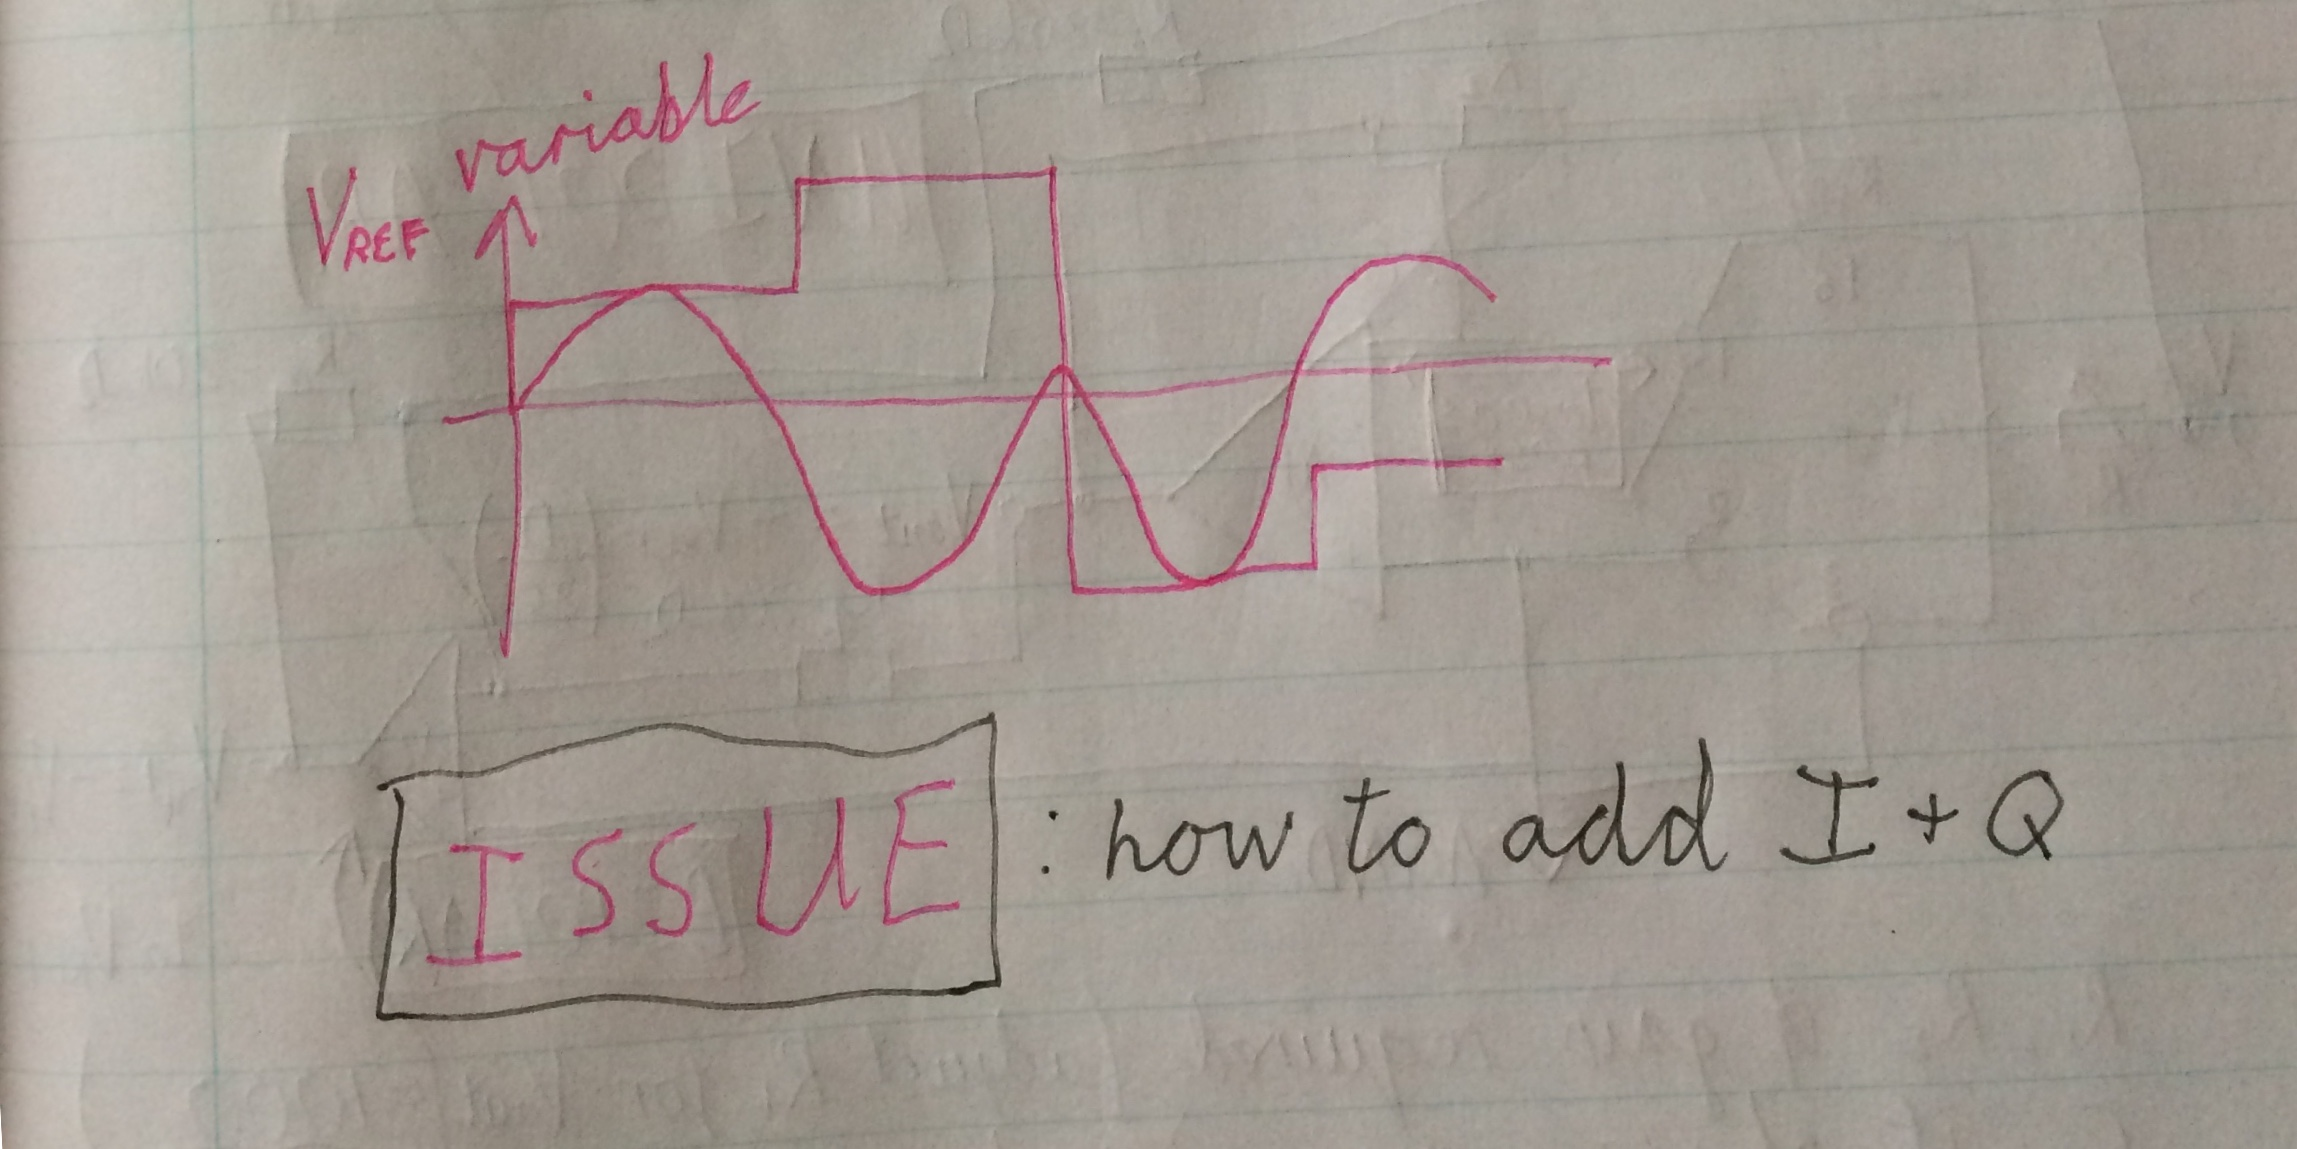
\includegraphics[width=0.6\textwidth]{DAC_Modulation.jpg}
	\caption{Four Quadrant Multiplication of input sinusoid using DAC}
	\label{fig_}
\end{figure}

The Pi is not able to output negative voltages.
As a result, Pulse Amplitude Modulation uses the range $0$ to $V_{max}$ rather than $-V_{max}$ to $V_{max}$.
Similarly, Quadrature Amplitude Modulation uses a grid of I and Q values all in the positive quadrant (0,1,2,3 not -3,-1,1,3).
The same "negative" effect is still achieved by using the "GROUND" of the multipliers (which are fully differential)
as $V_{max/2}$ using a voltage divider.
This means that the sine and cos signals would be inverted when multiplied by the values 0 and 1 in the same way they would be for -3 and -1, and the transmitted signal will essentially be a normal PAM or QAM signal plus a DC component of $V_{max/2}$.

\begin{figure}[ht]
	\centering
	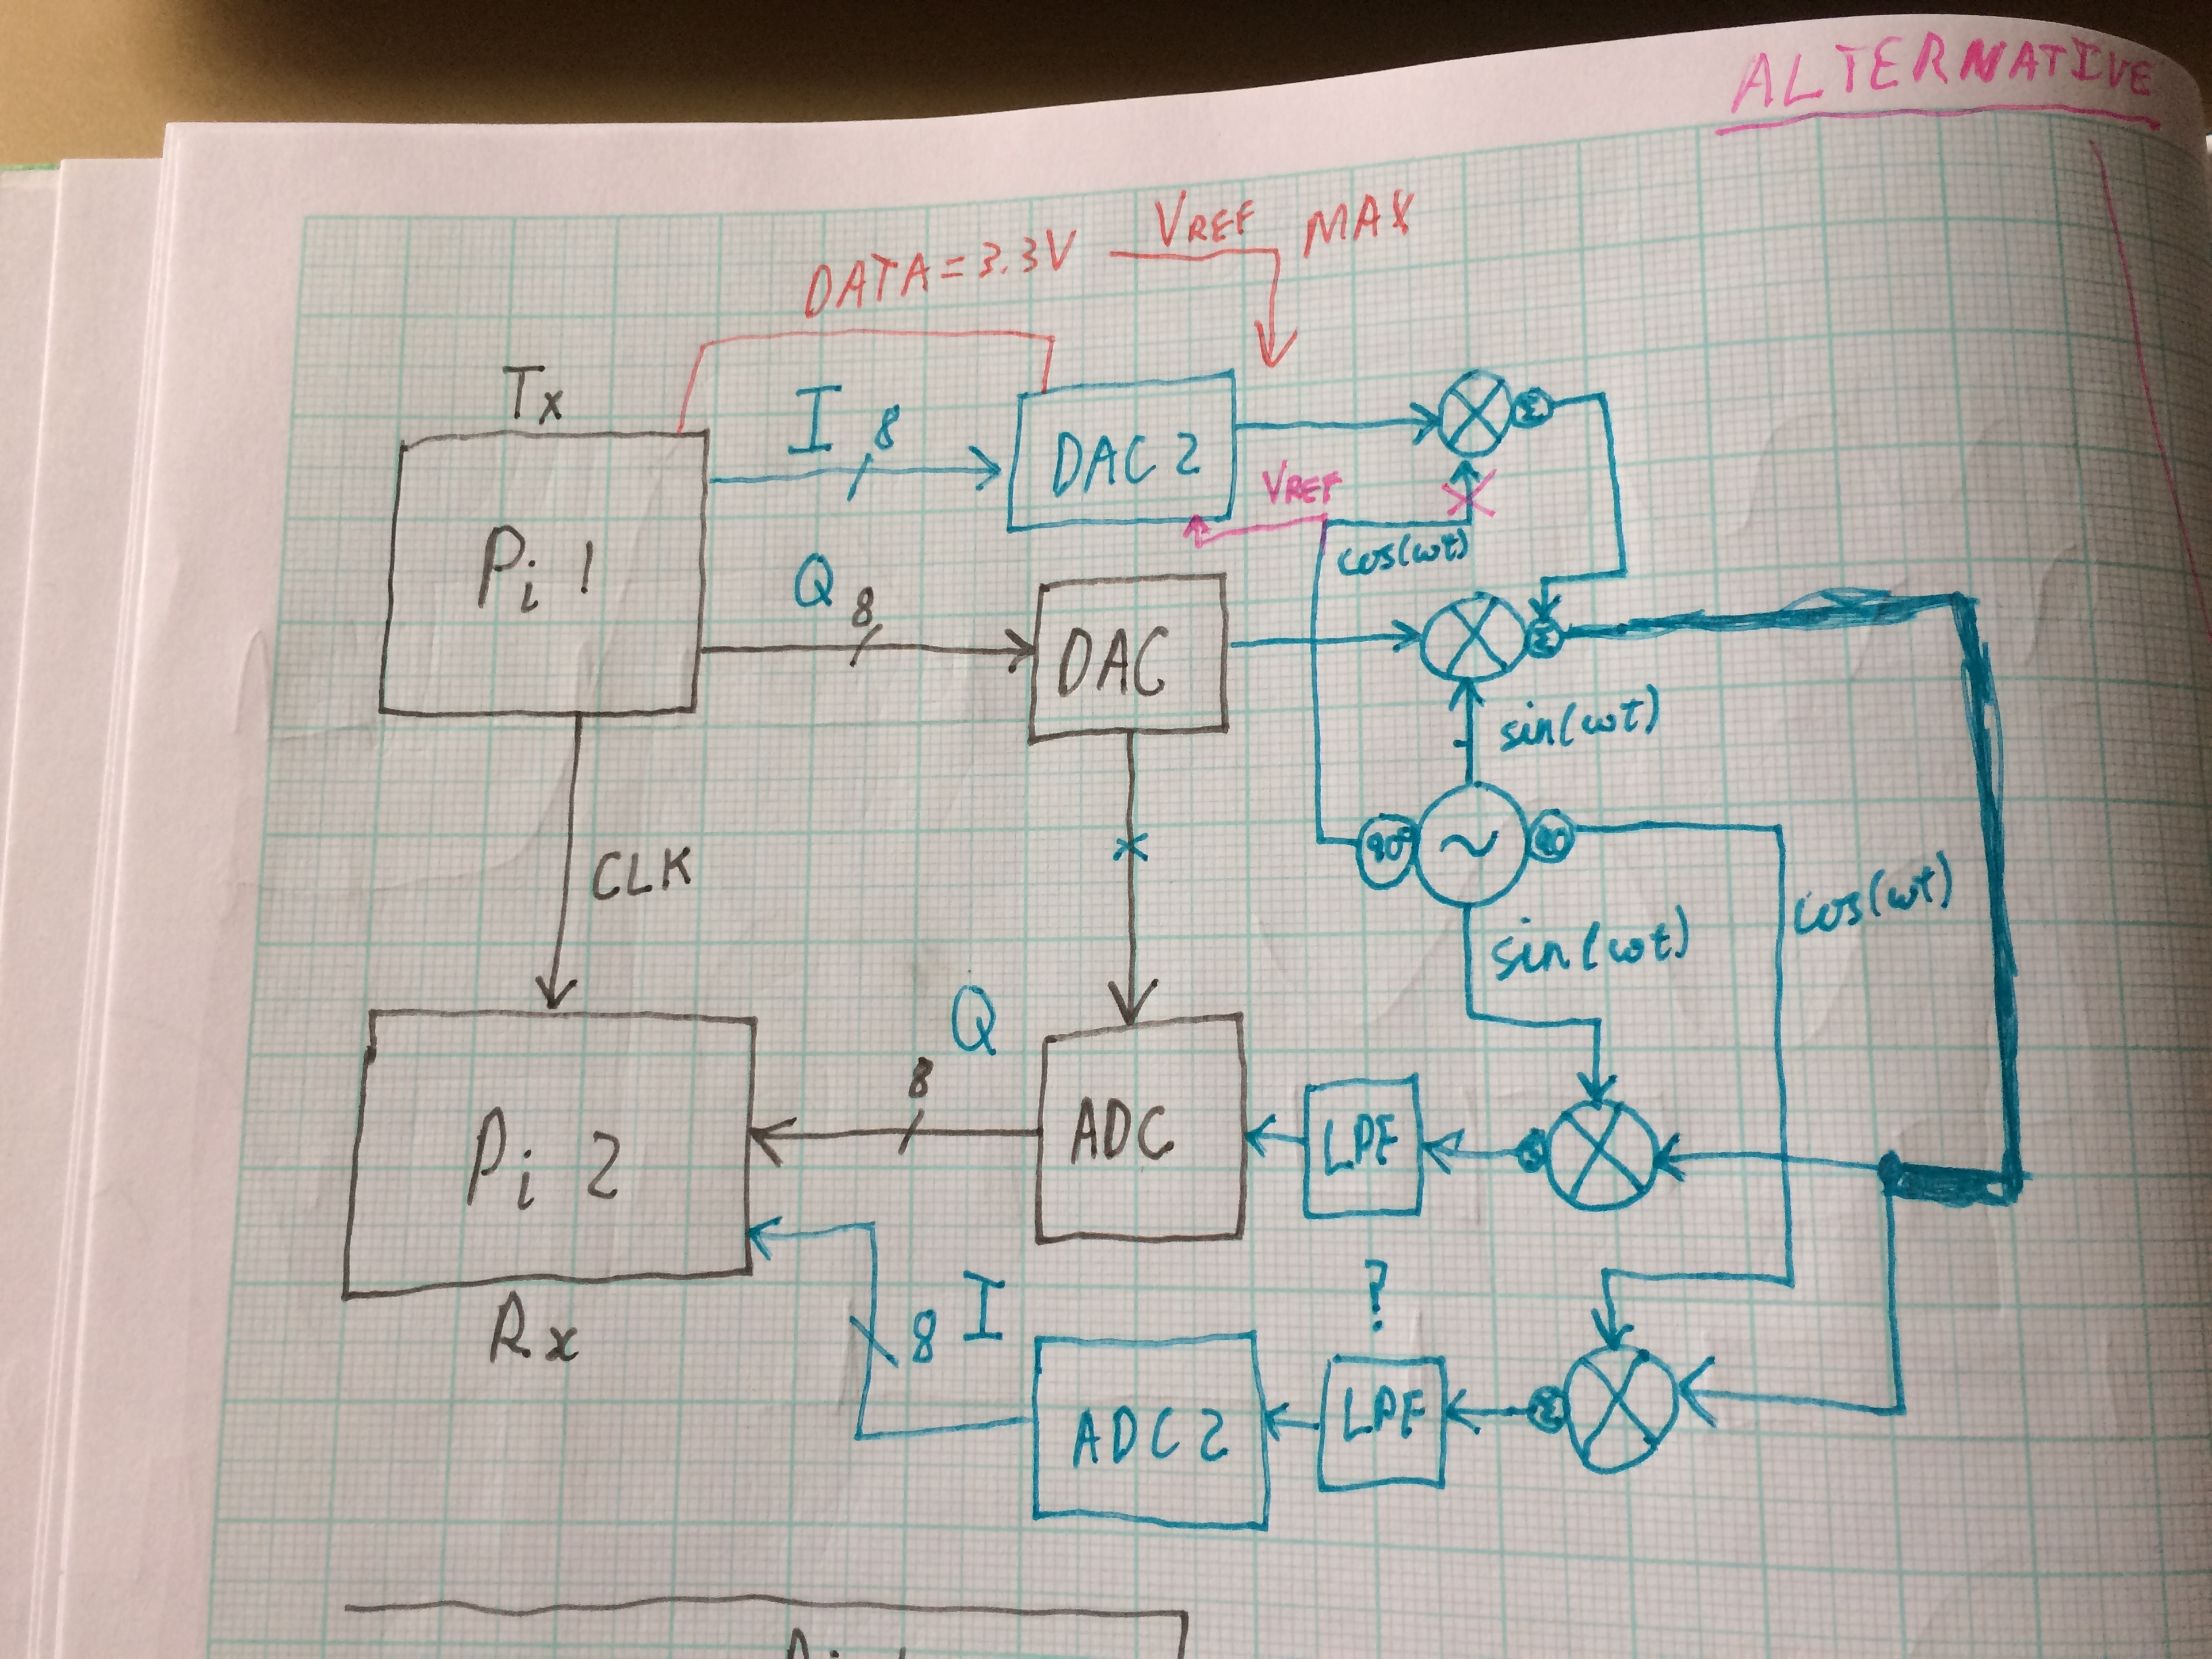
\includegraphics[width=0.6\textwidth]{QAM_OFDM_Architecture.jpg}
	\caption{Layout of the Test Bed for QAM and Potentially OFDM}
	%\label{fig_}
\end{figure}

\subsection{Parts Used}

\todo[inline,color=green!40]{Need a diagramatic representation of this as well as an actual picture of the final test bed}
\begin{figure}[ht]
	\centering
	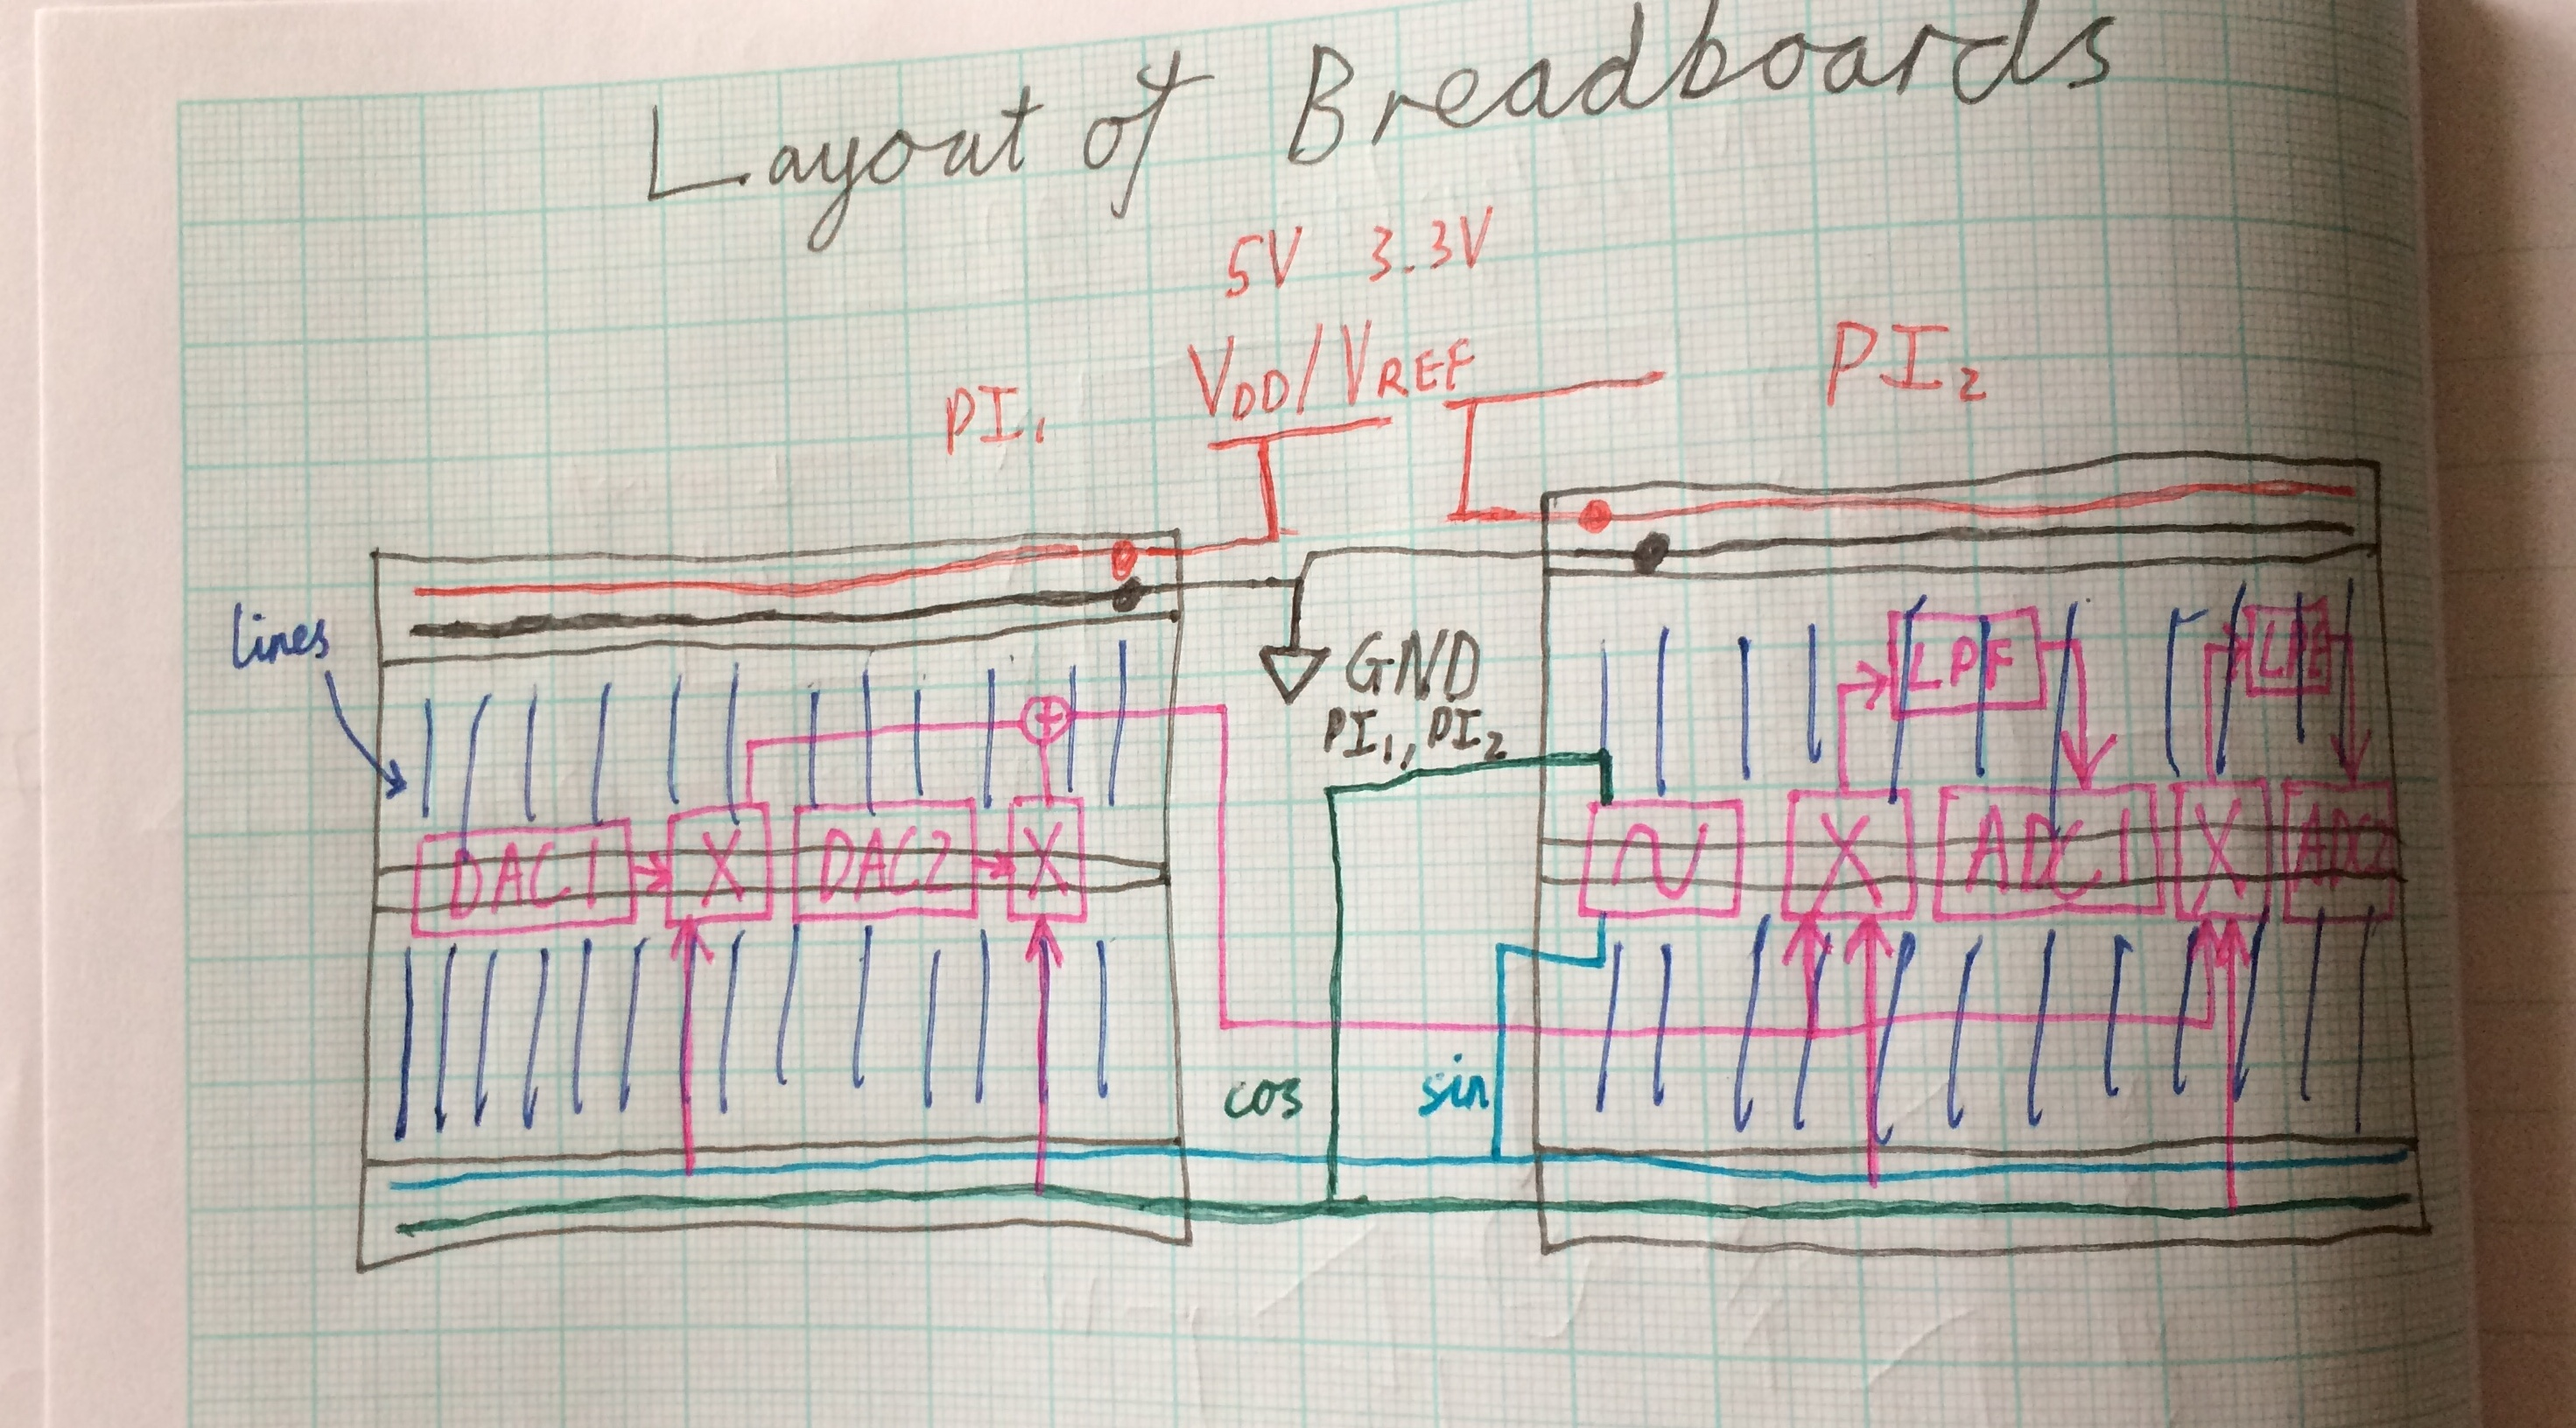
\includegraphics[width=0.6\textwidth]{Live_Test_Bed.jpg}
	\caption{The Final Configuration of the Test Bed}
	%\label{fig_}
\end{figure}

\todo[inline,color=blue!20]{Include a section on pricing of the parts and of the whole test bed, comparison to examples of projects and commercial solutions mentioned in Literature Review (Section \ref{sec_Lit Review})}

It is worth noting that there is a large variety of available options for each component of the test bed.
Each possibility has certain advantages and disadvantages, and a lot of the options are not suitable due to the power requirements or ease of interfacing with the Raspberry Pi.
As a result of this, the parts used in this project were the most suitable parts which could be found and successfully sourced.
However, there may be more suitable chips available given more time or experience to find them, and being aware of this would be useful if this project were to be extended and/or replicated.
All parts could be replaced with minimal adjustment to the physical test bed layout and code.\\

Changes which would be made with hindsight, if components with the required qualities could be found, are as follows:

\todo[inline,color=blue!20]{Continue to add to this list as you write the Architecture section - remove redundant information already discussed in the Section itself for each part}
\begin{itemize}
	\item A number of chips used are surface mounted, requiring difficult soldering to solder pads, This would be useful if they were to be used on a printed circuit board for a final design, but on a prototyping breadboard, dual in-line packages would have been easier to use where available
	\item The Digital Analogue Converter was chosen for its easy interfacing with a microcontroller, but a voltage-output device would remove the need to use additional operational amplifiers or a drain resistor at the output. It also had some issues with correct value output (See Section \ref{sec_Components}).
	\item Analogue Digital Converter
	\item The Quadrature Sinusoid Generator uses an oscillator chip which outputs $90^o$ out-of-phase square waves, and the chip used was the only simple one which did this or anything close. Ideally the outputs would already be sinusoidal (one quadrature chip or a sine generator and phase shifter) so that low pass filters with fixed frequency response could be omitted from the design, making the carrier frequency purely software-dependent. No obvious chip could be found for this and ones that did anything close were expensive.
	\todo[inline]{Make sure it's consistent with use of Quadrature Sinusoid Generator vs Oscillator in report}	
	\item The multiplier is designed to operate around \SI{10}{\volt}, and so has a built in \SI{10}{\volt} normalisation in the multiple which attenuates the signal (which is at lower voltages) and requires re-amplification before transmission - an oversight when choosing it. A similar chip designed for lower voltages would be ideal.
	\item Low Pass Filters to remove high frequency signals in the demodulation part of QAM were again made using fixed-value components, if frequency response of a filter could be altered in software, all frequencies used (carrier and symbol) could be hardware independent.
\end{itemize}

\clearpage

%%%%%%%%%%%%%%%%%%%%%%%%%%%%%%%%%%%%%%%%%%%%%%%%%%%%%%%%%%%%%%%%%%%%%%%%%%%%%%%%%%%%%%%%%%%%%%%%%%%%%%%%%%%%%%%%%%%%%%%%%%%%%%%%%%

\section{Programming}

The Raspberry Pi is used for its low cost, ease of use, and the fact that it has programmable Input/Output (I/O) pins.
The I/O pins can be programmed using different libraries in either Python or C.
The standard GPIO library which comes installed with Raspbian is RPi.GPIO for Python \cite{lib_RPi.GPIO}.
This is used for the On-Off Keying part of the communications test bed.
Python is relatively slow however, and so a C library is used for the pin-level manipulation for all modulation schemes requiring multi-pin outputs to Digital Analogue Converters to generate multi-level signals.
This is done both for the improved speed performance of the C library, and the capability of this library to output to multiple pins at once.
Section \ref{sec_Comparing Python and C} goes into a detailed  investigation of the differences between the libraries used and the reasons for choosing C over Python for the advanced modulation schemes.
All of the code and the report for the project are maintained on GitHub, and may be found at \url{https://github.com/CamEadie/4YP_PiCom}.\\

The transmitter and receiver code for all modulation schemes considered works from a single final version of the test bed code.
This comprises of the Python transmitter \textit{PiComTx\textunderscore 5\textunderscore DAC.py}, and receiver \textit{PiComRx\textunderscore 5\textunderscore DAC.py}, as well as the executables compiled from C code for the transmitter \textit{PiTransmit\textunderscore 3}, and receiver \textit{PiReceive}.
The main function in the Python files for each the transmitter and receiver is split into On-Off Keying and Advanced Modulation Schemes.
On-Off Keying (Section \ref{sec_On-Off Keying}) is the simplest form of clocked communication, and acts as a proof of concept for the Raspberry Pis as a test bed.
It is implemented using Python lists to store '1's and '0's to represent the binary stream.
These are output using the native RPi.GPIO library.\\

The OOK part was added into the final code for the Advanced Modulation Schemes (Section \ref{sec_Advanced Modulation Schemes})  from previous versions retrospectively, as all of the Advanced Schemes are implemented in the same code.
This was done to make it easier to conduct all communications tests through a single program interface.
It also allows all of the modulation schemes to be used on essentially the same layout with minor changes to the hardware, and this adheres better to the idea of Software Defined Radio being as software-defined and hardware-change-independent as possible (Section \ref{sec_Lit Review}).\\
\todo[inline,color=green!40]{Rephrase this and make sure the section referenced is as consistent with this comment as possible - reference that paper or lit review}

The advanced modulation schemes considered are 4-level Pulse Amplitude Modulation, 256-level Pulse Amplitude Modulation (used more for setting up the DAC and ADC, as differentiating between levels this precisely is not viable), 16-Quadrature Amplitude Modulation and Orthogonal Frequency Division Multiplexing.
Code for this section implements the data stream as bytes in a \textit{NumPy} array rather than as bits in a list.
This has certain computational advantages but also allows for the integration of image handling with \textit{imageio}.
This means that images can be transmitted instead of random data, allowing for visualisation of the bit error rate etc. of the transmission.
These schemes also use a separate compiled C module for the actual transmitting and receiving of data.\\

\begin{figure}[ht]
	\centering
	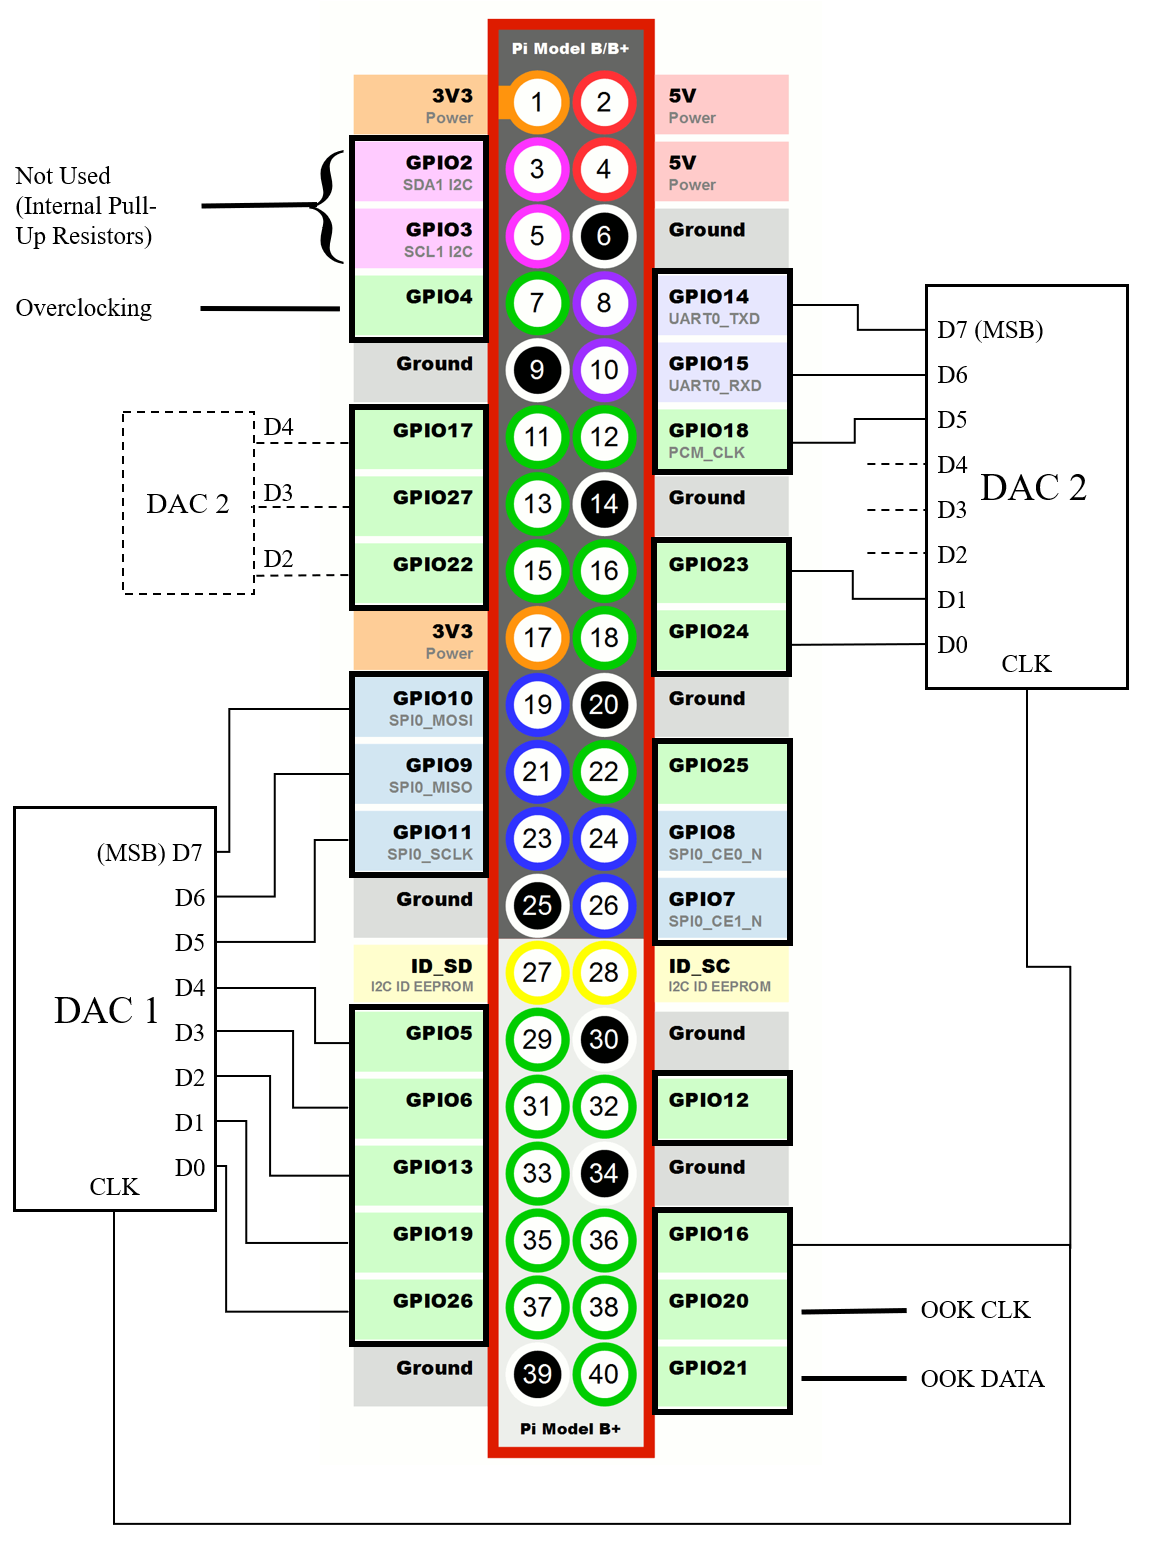
\includegraphics[width=0.8\textwidth]{Pi_Pin_Connections.png}
	\caption{Pin Diagram of Connections to Raspberry Pi (reference to image source) - These are alterable fairly easily in the code so changes can be made with little overhead}
	\label{fig_Pin Connections}
\end{figure}

Pins used currently for the OOK transmission as well as for the DACs are shown in Figure \ref{fig_Pin Connections}.
The pins with black boxes around them are the accessible GPIO pins, and they are referred to by their BCM number (GPIO\# in the boxes) rather than their BOARD number (consecutive numbers in the circles).
Of particular interest due to their differences are pins 2, 3 and 4.
Pins 2 and 3 are used for the clock and data lines of $I^2C$ bus communication and so have internal pull-up resistors.
Due to the fact that the test bed uses pins set with pull-down resistors, these pins aren't used.
Pin 4 is the only pin on the Raspberry Pi B+ with access to a hardware clock which can be programmed for external use.
It is thus used for overclocking external components which can be fed a clock signal, which is discussed in Section \ref{sec_Overclocking}.
The code defines the pins used for transmission as global variables at the start so that the rest of the code can be pin-independent.
Excepting the the DAC clock pin (pin 16) which is defined in the C code, Listing \ref{lst_Pins} shows these pin definitions.\\

\begin{lstlisting}[caption={Pins used for OOK and the DACs}, label={lst_Pins}]
	# OOK Pins
	CLK_PIN = 20
	DATA_PIN = 21
	# DAC Pins
	DAC_PINS_1, DAC_PINS_2 = [10, 9, 11, 5, 6, 13, 19, 26], \
								[14, 15, 18, 17, 27, 22, 23, 24]
\end{lstlisting} 

\subsection{On-Off Keying} \label{sec_On-Off Keying}

On-Off Keying is a modulation scheme based on using $V_{max}$ as '1' and \SI{0}{\volt} as '0'.
The transmit section of the test bed loops through the data list, outputting each value to the data pin followed by a clock pulse using the sleep function.
The speed and accuracy of the \textit{GPIO.output()} and \textit{sleep()} functions is covered in Section \ref{sec_Electro Testing}.
The receiver uses the function \textit{GPIO.wait\textunderscore for\textunderscore edge()} on rising edges of the clock pin to trigger reading of the data pin.
Using a function which is polling the clock pin as opposed to interrupt-driven solution is not ideal, but it was more easily written and so used for this early-stage modulation scheme.\\

Earlier versions of this modulation scheme included a function \textit{Prep\textunderscore Binary\textunderscore Data()} which added initial and final padding to the data of '1's to prevent missing timing of the beginning and end of transmission.
The function also added a padding bit to the data when either value had been repeated a certain number of times (for example a '1' if '0' had been repeated 5 times in a row).
This function was removed when \textit{Encode\textunderscore Error\textunderscore Correction()} was included, as forward error correction was seen as a better way of avoiding these and other errors without including padding bits which may be difficult to remove if errors did occur in the code transmission.
The channel coding used is syndrome decoding and is discussed more in Section \ref{sec_Channel Coding}.\\


\subsubsection{Starting the Receiver} \label{sec_SSH}

The receiver is started with the library Paramiko \cite{lib_Paramiko} which is used to make an SSH connection, and then to execute a command on the device which it connects to.
The host names of the transmitter and the receiver were changed to \textit{raspberrypi1} and \textit{raspberrypi2} to differentiate them, and their passwords changed to \textit{rasPass1} and \textit{rasPass2}.
The devices are connected by an Ethernet cable so no connection to the internet is required, and so the transmitter can use the local host name of the receiver \textit{raspberrypi2.local}.\\

The command to start the program is:

\begin{lstlisting}[caption=Command Line to Start the Receiver]
	command = "sudo python3 " + \
		"/home/pi/Documents/4YP_PiCom/4YP_PiCom_Receiver/PiComRx_5_DAC.py" + \
		" " +str(mask_length) + " " +str(TRANSMISSION_TYPE)
\end{lstlisting}

The super user call \textit{sudo} is necessary for control of the GPIO pins in the receiver code.
When programs are run from a command in command line mode, it can have additional information to it through the use of command line arguments.
These are additional space-separated strings after the name of the program which can be accessed by the program.
The command line argument \textit{mask\textunderscore length} is required by the receiver, and ensures that the amount of data received is the amount expected, and allows for the checking of deletions in the transmission.
The other argument \textit{TRANSMISSION\textunderscore TYPE} is not required, but if passed it overwrites the transmission type in the receiver code to ensure that it is expecting the same modulation scheme that the transmitter is using.\\

The SSH connection is closed as soon as the command is executed so that both Raspberry Pis are not expending resources during transmission, and any readout to \textit{stdout}, the standard output of the program over the connection is ignored.
All logging of the receiver is instead appended to a Python list \textit{LOGS}, and this variable is written to a file \textit{LOGS.txt} at the end of execution.
This includes all of the trivial to calculate results of the post-transmission analysis such as the number of bits/bytes received (whether there was any data lost).
\todo[inline]{Clearly check below once done}
The transmitter also implements another SSH connection after transmission to read the \textit{LOGS.txt} file to the \textit{stdout} of the connection using the command \textit{cat} so that the user does not need to change the screen (if only one screen available) between Raspberry Pis every time to see whether the transmission was successful.\\

\subsection{Advanced Modulation Schemes} \label{sec_Advanced Modulation Schemes}

\todo[inline,color=blue!20]{Write up notes in Advanced Modulation Schemes into a proper coherent section}

This section will start by describing the advanced modulation schemes used, and will then it will go on to how the transmitter and receiver implement  the schemes in code.\\

The modulation schemes used are 4-level Pulse Amplitude Modulation (4PAM), 256-level Pulse Amplitude Modulation (256PAM) and 16-Quadrature Amplitude Modulation (16QAM).
Orthogonal Frequency Division Multiplexing (OFDM) is discussed as a possibility but not implemented.
4PAM expresses each bit pair as one of four voltage levels which is expressed with use of a Digital Analogue Converter (DAC).
16QAM uses a similar concept except it transmits two voltages at once to describe each set of four bits.
This is achieved using two DACs, and by multiplying the output of one by a sine wave and the other by a cos (or $90^o$ phase-shifted sine) and adding them, using the orthogonality of the two waveforms to extract each level independently at the other end.
OFDM is a scheme which uses sub-carrier modulation in the digital domain, where each sub-carrier is modulated with a conventional modulation scheme such as Phase Shift Keying or QAM.
It then transmits the Inverse Fast Fourier Transform (IFFT) of the combination of these sub-carriers as a complex carrier-modulated signal.\\

The communications test bed could be implemented with OFDM, however there were certain issues and time constraints which meant that this was not realised.
The details of how the test bed would be extended are included.
As mentioned in Section \ref{sec_Multiplier}, the Raspberry Pi is unable to output negative voltages, and so all symbol values are in a positive voltage range between $V_{min} = 0V$ and $V_{max} = 3.3V$.
Therefore, 4PAM and 16QAM use values from the range $\{0, 1, 2, 3\} \times \frac{3.3}{3}V$, output from one and two DACs respectively.
Similarly 256PAM uses 256 values from $\{0, 1, ..., 255\} \times \frac{3.3}{255}V$.\\

\newpage

Figure \ref{fig_Transmitter_Flow} (see Page \pageref{fig_Transmitter_Flow}) is a flow chart of the operation of the transmitter code.
256PAM is omitted in the flow chart as it is similar to but more easily realised than 4PAM, and the space is better used conceptualising the addition of OFDM.
256PAM is also not a viable modulation scheme unless the DAC acts perfectly, and so it is implemented mostly as a way of testing the accuracy of the DAC's granularity.
Tests using 256PAM to output monotonically increasing values revealed that the converters were not working exactly as expected, and that there were spikes at certain values and a non-continuous analogue response was measured for continuous digital input.
This problem is investigated in Section \ref{sec_Components}, but the solution was to use an empirically derived lookup table to get the four levels for 4PAM and 16QAM as close as they could be to the correct values -- this would be removed from the code if a successful replacement digital analogue converter was used.\\
\todo[inline,color=green!40]{Make sure the corresponding section (USE THE RIGHT SUB-SECTION) does reference the fact that the DAC doesn't work exactly as it's supposed to and how I dealt with it}

\begin{figure}[ht]
	\centering
	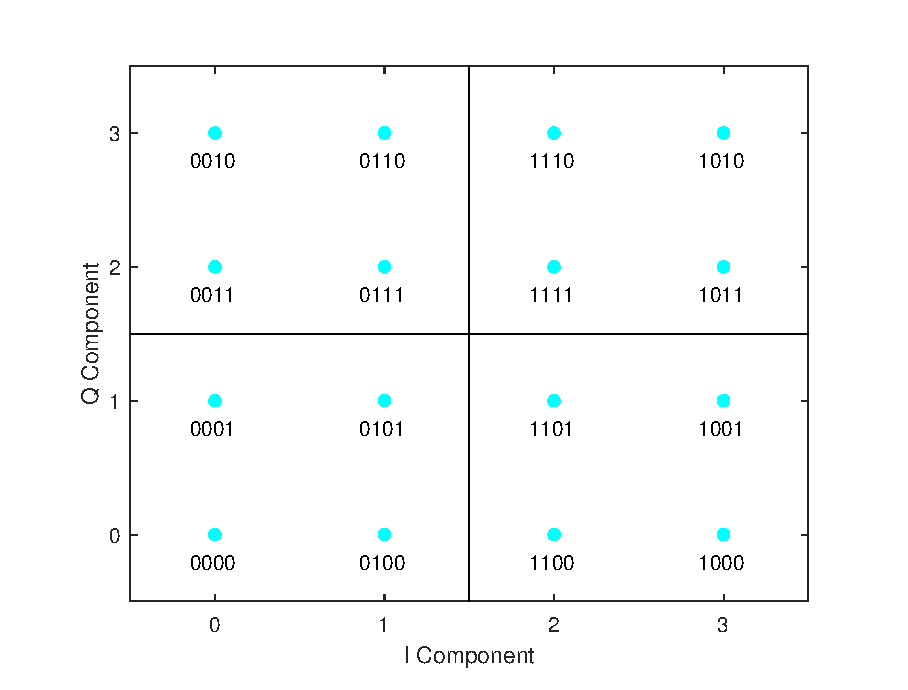
\includegraphics[width=0.8\textwidth]{QAM_Const.eps}
	\caption{16-QAM Constellation with Grey Code}
	\label{fig_QAM Constellation}
\end{figure}

The transmitter can be run from the command line with transmission frequency and modulation scheme as command line variables, otherwise it uses the currently coded in values.
For 4PAM, each byte is split into four symbols, and each symbol (of value 0, 1, 2 or 3) is converted into an 8-bit digital value.
As mentioned above this is done with a lookup table, but would ideally be done by multiplying each symbol by $\frac{255}{3} = 85$.
The values are then expanded into bitmasks which can be used by the bank write operation in the C code.
This is explained in below in Section \ref{sec_C Transmitter and Receiver}.
For 16QAM each byte is split into two symbols, where each symbol consists of an I and a Q component (of value 0, 1, 2 or 3).
These symbols are chosen using the grey coded 16QAM constellation in Figure \ref{fig_QAM Constellation}.
Grey code is a binary system where any symbol has only one bit difference to all directly adjacent symbols, and it is chosen because if a symbol is incorrectly decoded, the next most likely symbols are directly adjacent and so only one bit will be incorrect, minimising the bit error.
By inverting the constellation, a dictionary of 4-bit values to symbols is used to easily convert each byte to two symbols.
This is done by unpacking each byte into corresponding bits and reshaping into a matrix with four columns, then each row is taken as a dictionary key to decode the symbol, shown in Listing \ref{lst_Inverted QAM}.
Each symbol is then converted into an 8-bit DAC value and expanded onto a bitmask for the C code, with the I component mapped to the first DAC's pins, and the Q component mapped to the second DAC's pins.\\

\begin{lstlisting}[caption={Inverted QAM Constellation and its use to encode each byte as two symbols}, label={lst_Inverted QAM}]
	mapping_table = {
	(0,0,0,0) : 0 + 0j,
	(0,0,0,1) : 0 + 1j,
	(0,0,1,0) : 0 + 3j,
	(0,0,1,1) : 0 + 2j,
	(0,1,0,0) : 1 + 0j,
	(0,1,0,1) : 1 + 1j,
	(0,1,1,0) : 1 + 3j,
	(0,1,1,1) : 1 + 2j,
	(1,0,0,0) : 3 + 0j,
	(1,0,0,1) : 3 + 1j,
	(1,0,1,0) : 3 + 3j,
	(1,0,1,1) : 3 + 2j,
	(1,1,0,0) : 2 + 0j,
	(1,1,0,1) : 2 + 1j,
	(1,1,1,0) : 2 + 3j,
	(1,1,1,1) : 2 + 2j }
	# Unpack data list into N bits and reshape to (N/4 x 4) bit matrix
	data_list_bits = np.unpackbits(data_list)
	data_list_bits = data_list_bits.reshape( (data_list_bits.size//4, 4) )
	# Convert (N/4 x 4) matrix into N/4 symbols
	def Mapping(bits):
		return np.array([mapping_table[tuple(b)] for b in bits])
	symb = Mapping(data_list_bits)
\end{lstlisting}

OFDM is also conceptualised here but due to the DAC continuous value issue mentioned above, a better-functioning DAC would need to be found before this could be implemented.
For OFDM, the data stream is split into N sub-streams, each transmitted on a separate sub-carrier.
These sub-carriers are chosen to be orthogonal so they do not interfere with each other, normally achieved by having each sub-carrier centred at integer multiples of the desired frequency gap $\delta F$.
The transmitter takes N complex symbols from the conventional modulation scheme - 16QAM for example - at a time, and puts them through an IFFT  with N inputs.
The complex output is then transmitted as a complex carrier-modulated signal, meaning that the real output of the IFFT would be modulated by a sine wave and the imaginary output by a cos wave at a chosen carrier frequency in the same manner as the I and Q components of QAM.
NumPy has functions \textit{numpy.fft()} and \textit{numpy.ifft()} which make the transition from 16QAM to OFDM as simple as splitting the signal into multiple streams before converting the data into QAM symbols, and then using the symbols as inputs to the IFFT.
Adding a cyclic prefix to each block of IFFT samples to prevent inter-block interference, ensuring the outputs are expressed as 8-bit digital outputs and mapping the values to a set of bitmasks would still need to be included.\\

For all modulation schemes considered, once the output is expressed as an array of bitmasks - essentially 32-bit binary numbers where each bit corresponds to a pin to set - each element in this array is exclusive bitwise OR-ed (XOR-ed) with the bit mask of the two DACs' address pins.
This results in another array of bitmasks where all of the pins in the DAC bitmasks are inverted, and all the other pins remain zero.
This is necessary because the C library has two bank operations (which work on a bank of pins), \textit{gpioWrite\textunderscore Bits\textunderscore 0\textunderscore 31\textunderscore Set()} and \textit{gpioWrite\textunderscore Bits\textunderscore 0\textunderscore 31\textunderscore Clear()}.
As the name suggests, one is required to set all of the pins which will be set to '1', and one is required to clear all of the bits which will be set to '0' but may have been '1' before.
Both arrays are saved as binary files, so they can be read in by the C transmitter code.
At this point the command to start the receiver is passed through an SSH link to the receiver and the connection is terminated.
The receiver is started with command line arguments of number of masks (symbols) and the transmission type.
After this, the C transmitter is started with one command line argument, mask (symbol) transmission frequency, otherwise known as baud rate.
The C transmitter sets up the pins for the transmission, reads in the binary files corresponding to the \textit{Set} and \textit{Clear} bitmasks, and then loops through, outputting the values to the DACs at the specified baud rate.\\

\begin{figure}[ht]
	\centering
	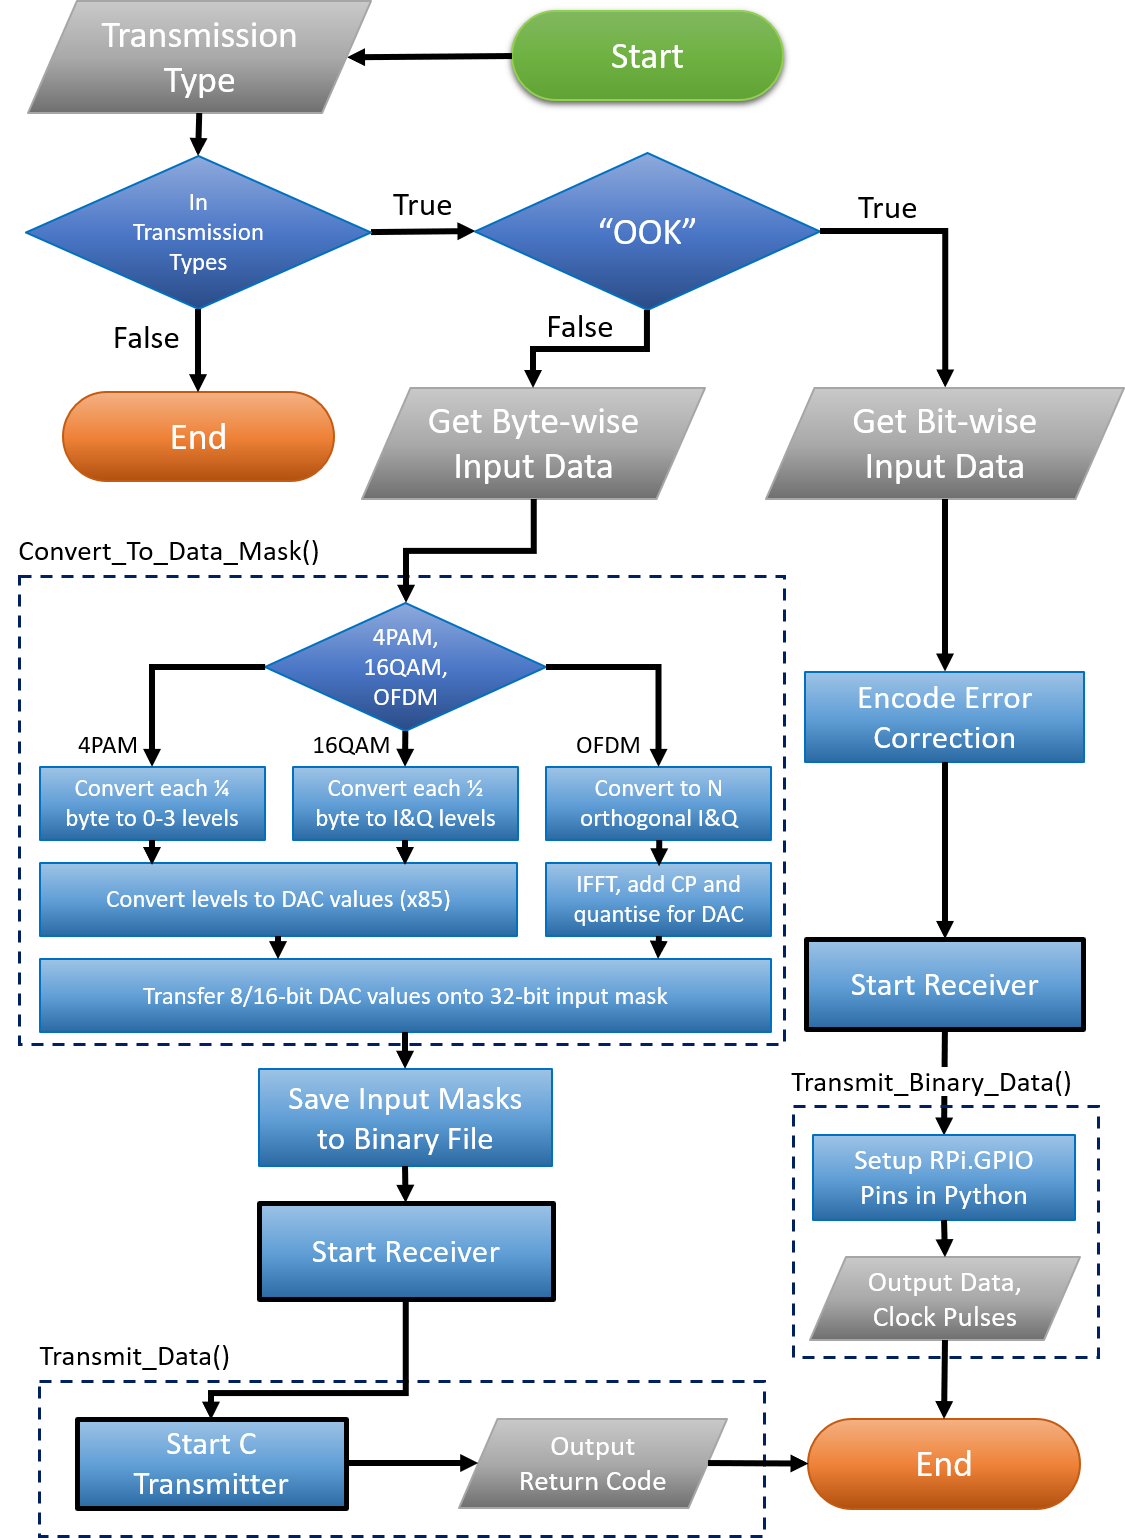
\includegraphics[width=\textwidth]{Transmitter_Flow.png}
	\caption{Flow Chart for Transmitter Code}
	\label{fig_Transmitter_Flow}
\end{figure}


\clearpage

Figure \ref{fig_Receiver_Flow} (see Page \pageref{fig_Receiver_Flow}) is a flow chart of the receiver code's execution path.
The receiver starts, and if the transmission type is not OOK and thus an advanced modulation scheme, it immediately starts the C receiver code passing the command line argument of number of masks so that it knows how much data to expect.
This part of the receiver saves one bitmask per clock pulse until it has received the expected amount of data.
There is also a way of checking if the transmission has finished, when the clock stops, so that if data was missed at the beginning of or during the transmission, the receiver will still stop listening and complete execution.
The C code then saves the bitmasks received to a binary file and terminates successfully.\\

If the C receiver is successful, the binary file is read into a NumPy array to be decoded.
For all modulation schemes, the first step is to de-map the data from the masks to their DAC value(s) using the list \textit{DAC\textunderscore Pins\textunderscore 1} as well as \textit{DAC\textunderscore Pins\textunderscore 2} for quadrature-carrier modulation schemes.
The receiver then measures the peak values of the signal and if there has been any attenuation of the signal, it is scaled to the full input range and the attenuation is logged.
PAM and QAM then use maximum likelihood decoding to figure out the correct symbol values.
This equates to using partitions which are half way between possible symbols to decode them.
For example in 16-QAM, any value within the box around each symbol in Figure \ref{fig_QAM ML Decoding} would be mapped to the symbol at its centre.

\begin{figure}[ht]
	\centering
	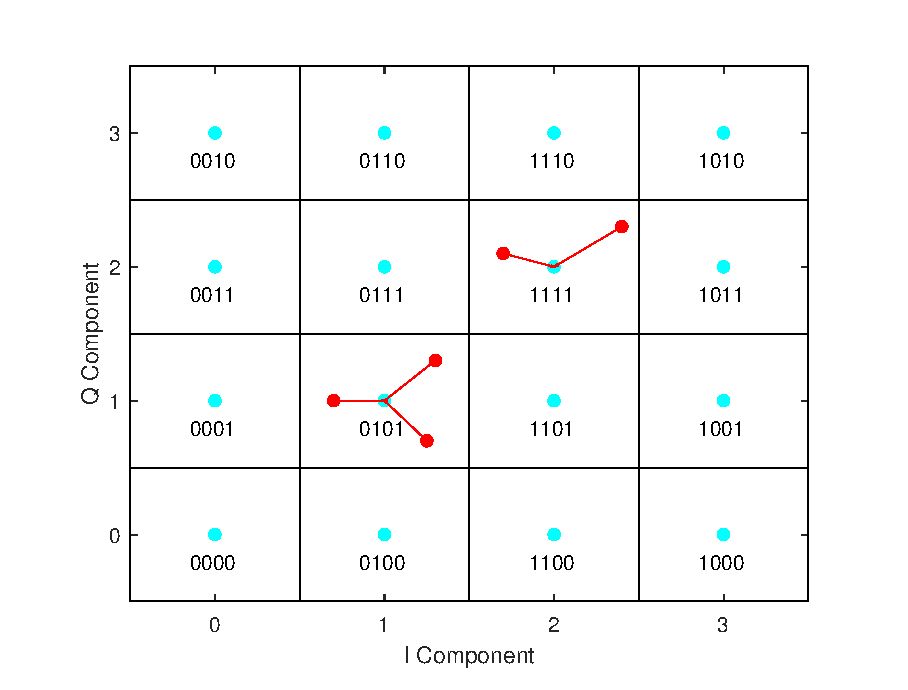
\includegraphics[width=0.8\textwidth]{QAM_Grid.eps}
	\caption{16-QAM Constellation with Maximum Likelihood Boundaries}
	\label{fig_QAM ML Decoding}
\end{figure}

\begin{figure}[ht]
	\centering
	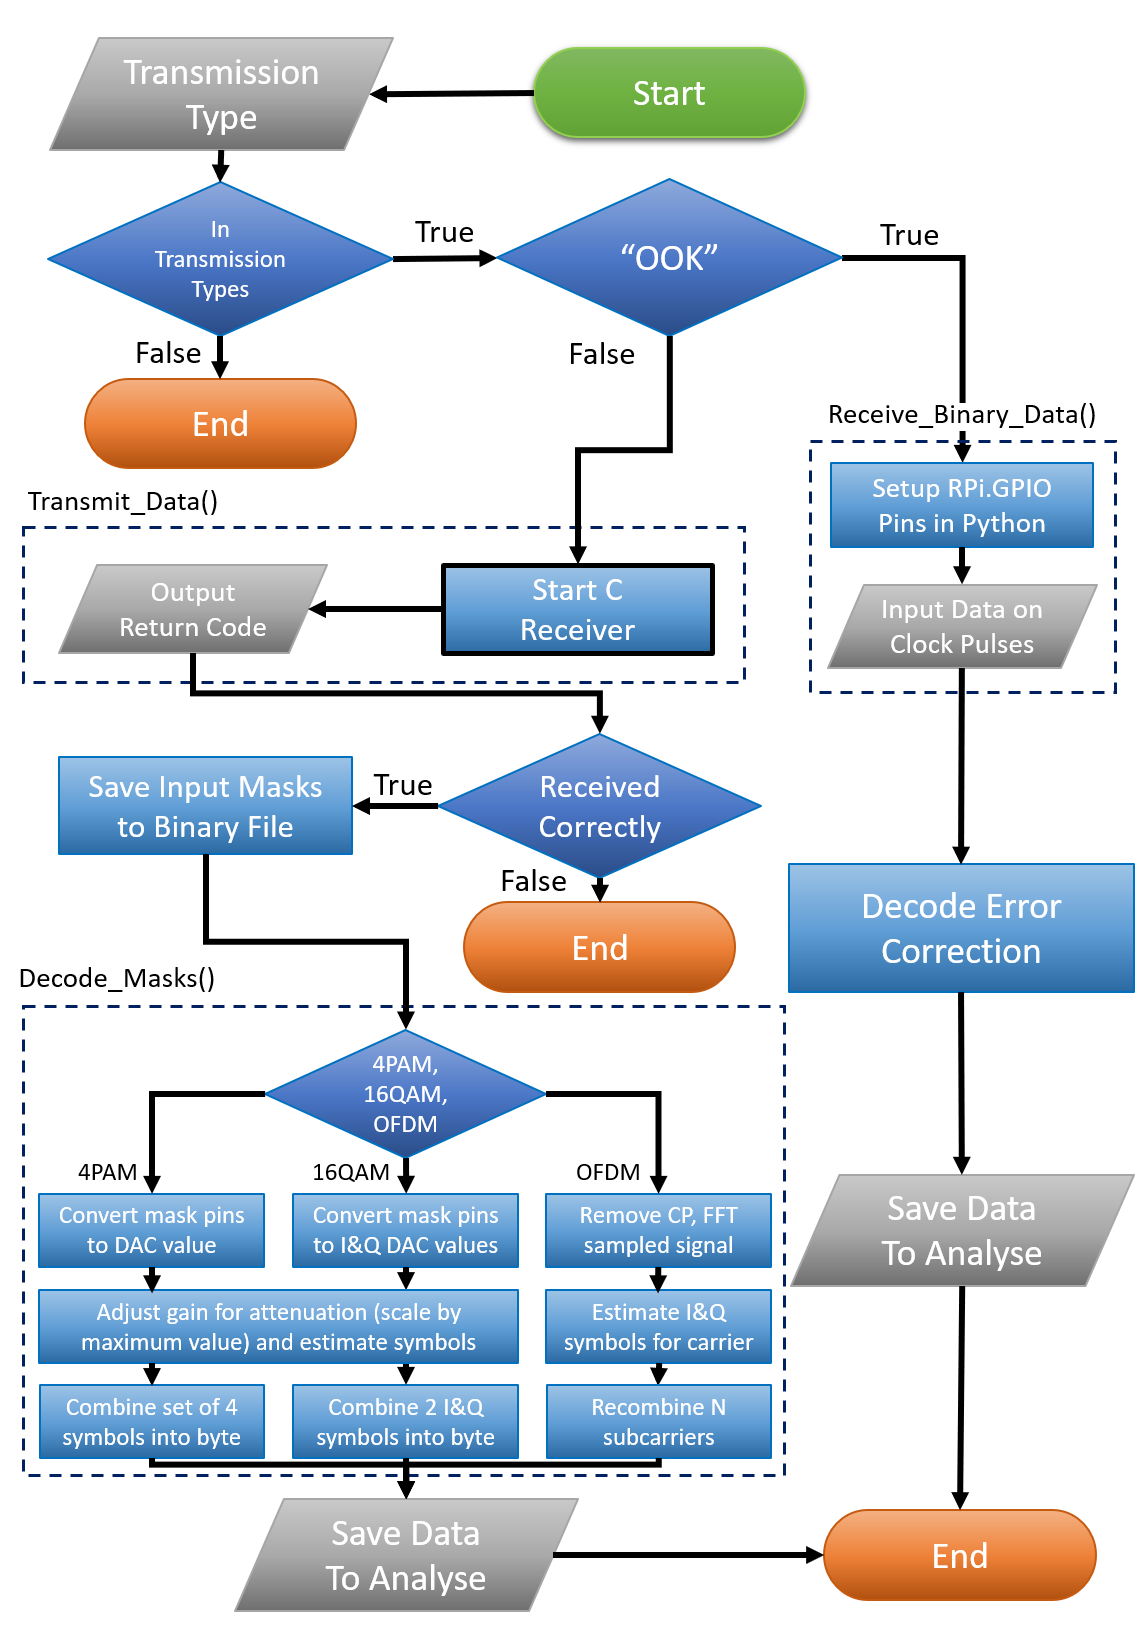
\includegraphics[width=\textwidth]{Receiver_Flow.png}
	\caption{Flow Chart for Receiver Code}
	\label{fig_Receiver_Flow}
\end{figure}


\todo[inline,color=blue!20]{Write the rest of receiver, Data and Image handling and the C Sections (and if time, the test masks code)}

\subsubsection{Data and Image Handling}

NumPy and imageio, how they work and are used in the code, examples.\\

\subsubsection{C Transmitter and Receiver} \label{sec_C Transmitter and Receiver}

Receiver: in Section \ref{sec_Computation} the options of data mask in on trigger vs read data then in on clock were compared and BLA was chosen as the more effective method.
\todo[inline]{Which method is more effective?}

PiTransmit works independent of the choice of DAC pins.
It reads in the bitmask (bits to set) from a binary file for speed, which is calculated and saved in the Python before transmission, and it also reads in inversion mask (bits to clear) so the calculation is not done during transmission.
This also means the Transmit program does not need to know how many DACs there are so works for all transmission schemes.

The pins selected are based on the DAC1 choice from Figure \ref{fig_Pin Connections} (reference already used) but could be used for any set of possible output pins.
There will also be an explanation about what these bitmasks actually mean and refers to, it is exemplified in Figure \ref{fig_Mask Expansion}.

\begin{figure}[ht]
	\centering
	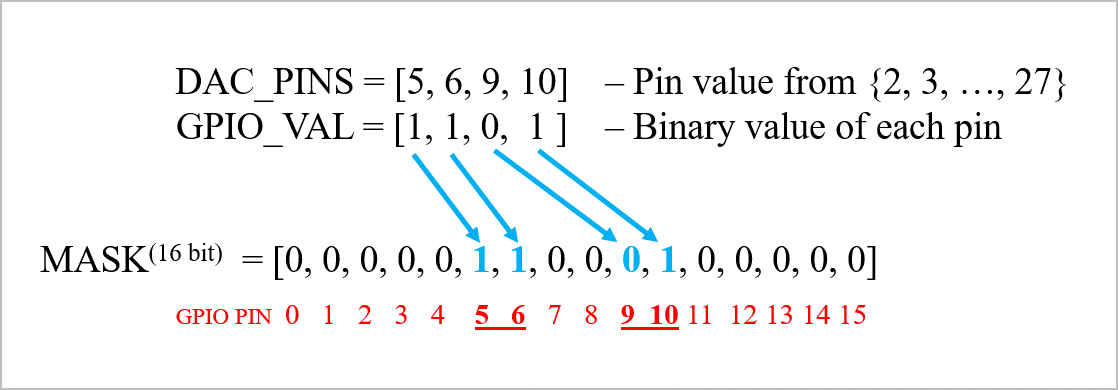
\includegraphics[width=0.8\textwidth]{Mask_Expansion.png}
	\caption{Explanation of the concept of mask expansion}
	\label{fig_Mask Expansion}
\end{figure}

\end{document}